% Created 2023-05-28 Sun 20:52
% Intended LaTeX compiler: pdflatex
\documentclass[a4paper, titlepage, twoside]{article}
\usepackage[utf8]{inputenc}
\usepackage[T1]{fontenc}
\usepackage{graphicx}
\usepackage{longtable}
\usepackage{wrapfig}
\usepackage{rotating}
\usepackage[normalem]{ulem}
\usepackage{amsmath}
\usepackage{amssymb}
\usepackage{amsfonts}
\usepackage{capt-of}
\usepackage{hyperref}
\renewcommand*{\thefootnote}{\fnsymbol{footnote}}
\pagestyle{headings}
\usepackage{microtype}
\usepackage{svg}
\renewcommand{\baselinestretch}{1.2}
\usepackage[margin=1.4in]{geometry}
\usepackage[font={small}, labelfont={}]{caption}
\usepackage{minted}
\usemintedstyle{vs}
\setminted{frame=single, framesep=2mm}
\usepackage{authblk}
\author{Konstantinos Chousos\thanks{Student ID: 1115202000215}}
\author{Konstantinos Kordolaimis\thanks{Student ID: 1115202000091}}
\author{Anastasios-Phaedon Seitanidis\thanks{Student ID: 1115202000179}}
\author{Aggelos Tsitsoli\thanks{Student ID: 1115202000200}}
\affil{Department of Informatics and Telecommunications, \\ National \& Kapodistrian University of Athens}

%% ox-latex features:
%   !announce-start, bibliography-biblatex, !guess-pollyglossia,
%   !guess-babel, !guess-inputenc, caption, maths, image, rotate,
%   bibliography-biblatex-resources, !announce-end.

\usepackage[backend=biber, style=alphabetic]{biblatex}


\usepackage{capt-of}

\usepackage{amsmath}
\usepackage{amssymb}

\usepackage{graphicx}

\usepackage{rotating}

\addbibresource{bibliography.bib}
\addbibresource{/home/kchou/Textfiles/biblio.bib}

%% end ox-latex features

\AtEveryBibitem{\clearfield{pagetotal}}
\usepackage{lmodern}
\usepackage{tabularx}
\setcounter{secnumdepth}{3}
\author{Konstantinos Chousos}
\date{May 26th, 2023}
\title{An In-Depth Analysis of Haskell\\\medskip
\large K31 Compilers, Spring 2023}
\hypersetup{
pdfauthor={Konstantinos Chousos},
pdftitle={An In-Depth Analysis of Haskell},
pdfkeywords={},
pdfsubject={},
pdfcreator={Emacs 29.0.90 (Org mode 9.7-pre)},
pdflang={English},
colorlinks,
linkcolor=blue,
citecolor=red,
urlcolor=blue}\begin{document}

\maketitle

\pagenumbering{roman}

\setcounter{tocdepth}{2}
\tableofcontents

\listoflistings
\listoftables

\renewcommand*{\thefootnote}{\arabic{footnote}}

\begin{abstract}
This report provides an in-depth look at the functional programming language Haskell. The first part covers the background of the language including its history and popularity, as well as its general position in the history of functional programming. It also delves into the various tools written in Haskell and its use cases in the tech industry. In the second part, control structures, laziness, identifiers, keywords, operators, lambdas, monads, memory management, namespaces, parallel programming, metaprogramming, and object-oriented properties of Haskell are discussed. The report concludes with several examples and code snippets, including a ``Hello, World!'' program and a factorial implementation.
\end{abstract}

\pagenumbering{arabic}
\setcounter{page}{2}

\section{Introduction}
\label{sec:org8ec6036}

\subsection{History of Haskell}
\label{sec:org10e55ee}

Haskell was born in the 1980's. It was a child of necessity. Its purpose was to be the answer to an ever-growing problem: The plethora of functional programming languages, among which there were enough differences to distinguish them, but not enough for any one to be unique enough \autocite{marlowHaskell2010Language2010}. This led to functional programming being discarded all together by many, as there didn't exist any kind of common ground between the different languages and implementations. Haskell's goal was --- and still is --- to be the pinnacle of the functional programming space. A language that would embody the functional programming principles and with capabilities suitable for real-world applications.

\subsubsection{Prehistory}
\label{sec:org3b6f381}

Functional programming first started gaining popularity around 1978, when John Backus --- the leader of the team that developed Fortran \autocite{backusFORTRANAutomaticCoding1957} and the inventor of the Backus Naur Form (BNF) --- published the famous \emph{``Can Programming Be Liberated from the von Neumann Style?''} lecture \autocite{backusCanProgrammingBe1978}. It presented functional programming as something useful in real world situations and applicable to tangible problems, as opposed to simply an academic and theoretical tool.

That's not to say functional programming was new. In fact, it had been around for at least 30 years at the time. Some important milestones in its history are the following:

\begin{itemize}
\item 1950's

John McCarthy created Lisp \autocite{mccarthyRecursiveFunctionsSymbolic1960}, which was the pioneering high-level functional programming language at the time, during his time at the Massachusetts Institute of Technology in the 1950s. The definition of Lisp functions involved the use of Alonzo Church's lambda notation (see \hyperref[sec:org04d0fd3]{Functional programming and lambda calculus}), which was expanded to enable the creation of recursive functions. Lisp was the first functional programming language to present several new exemplary features in the functional programming world. Lisp merged them, and as a result enabled the support of multiple programming styles. Subsequent dialects of LISP --- e.g Common Lisp, Racket, Scheme and Clojure \autocite{steeleCOMMONLISPLanguage1984,felleisenRacketManifesto2015,abelsonRevisedReportAlgorithmic1998,hickeyHistoryClojure2020} --- aimed to streamline LISP and make an easier version of it by emphasizing a purely functional foundation.

At the same time period another functional programming language was created with the name Information Processing Language (IPL) from Allen Newell, Cliff Shaw and Herbert A. Simon \autocite{newellIntroductionInformationProcessing1960}. IPL was created with the primary purpose of handling lists of symbols, enabling dynamic memory allocation and multitasking. It was the inventor of the concept of list processing.

\item 1960's

During the early 1960's, Kenneth E. Iverson was responsible for developing APL \autocite{iversonProgrammingLanguage1962}. APL primarily revolved around arrays that are multidimensional. By utilizing a wide variety of unique graphic symbols, APL enabled the creation of incredibly succinct code. APL and its creation was the inspiration for the development of other languages in later years e.g. the programming language K which was created in the 1990's by Arthur Whitney.

During the mid-1960's, Peter Landin played a key role in the development of functional programming languages. He was responsible for the creation of the SECD machine \autocite{landinMechanicalEvaluationExpressions1964}. In addition to creating the SECD machine, Peter Landin recommended the ISWIM programming language \autocite{landinNext700Programming1966}.

\item 1970's

During the 1970's, several functional programming languages were developed in Scotland. Robin Milner was the creator of ML. David Turner was responsible for the creation of SASL. Also at that period in Edinburgh, Burstall and Darlington created the NPL which was a functional programming language that utilized Kleene Recursion Equations \autocite{darlingtonProgramTransformationSynthesis1977}. Later, the previous two developers with Sannella implemented polymorphic type checking from ML into Hope, a language inspired by NPL. As time passed, ML evolved into some new idioms, with OCaml being one of the most popular.

Another functional programming language that was developed at that time was Scheme by Gerald Jay Sussman and Guy L. Steele \autocite{abelsonRevisedReportAlgorithmic1998}. Scheme was the initial variation of Lisp that mandated optimization in functions calls, which were recursive and happened in the rear position, also implemented lexical scoping.

It was at this time that John Backus's lecture was published \autocite{backusCanProgrammingBe1978}. He described functional programs as being constructed hierarchically using ``combining forms''. This type of construction was inspired from the principle of compositionality.

\item 1980's

During the 1980's, the intuitionistic type theory, developed by Per Martin-Löf, established a connection between functional programs and constructive proofs (these were expressed through dependent types).That opened up new avenues for collaborative theorem proving and had a significant impact on the evolution of later functional programming languages.

David Turner created the lazy functional language Miranda \autocite{turnerMirandaNonstrictFunctional1985} in the mid 1980's. This language in particular had a significant impact on the development of Haskell (see \hyperref[sec:orgcf67d8b]{Haskell and Miranda}).
\end{itemize}

\paragraph*{Functional programming and lambda calculus}
\label{sec:org04d0fd3}

In 1932 and 1933, mathematician Alonzo Church published two papers both titled ``A Set of Postulates for the Foundation of Logic'' \autocite{churchSetPostulatesFoundation1932,churchSetPostulatesFoundation1933}. In those papers a new formal system of mathematical logic was introduced that centered around the notion of functions, with the name of \emph{lambda calculus}. The purpose of using this framework was to represent calculation through function generalization and application, using binding between variables and variable substitution. Functional programming was invented as a practical application of lambda calculus, in order to benefit from its many uses.

It is known that lambda calculus was the basis for a lot of functional programming languages. Specifically, it gives a foundation for comprehending the nature of functions and it also provides the ability of combining many functions together to create a new function (also known as function composition). Functional programming employs functions as the essential units for constructing programs, and lambda calculus furnishes a means to precisely declare and contemplate these functions \autocite{pandaquestsRelationshipLambdaCalculus2023}.

Also, lambda calculus characterizes a function as a statement that accepts an input and generates an output. Their definition is based on lambda abstractions. Lambda abstractions are nameless functions that connect a variable to a calculation. Also they are employed to represent functions. 

Many languages such as Haskell were directly influenced by lambda calculus. The former offers tangible realizations of the concepts introduced by the latter. For instance, using lambda expressions you can create functions and you can combine functions through higher-order functions.

\paragraph*{The \emph{lazy} craze}
\label{sec:org9b8cdcf}

1970--1980 was a time period in which \emph{lazy evaluation} (see \ref{sec:org18a698d}) was getting more and more attention. It had been independently invented at least three times and there were many tries in implementing programming languages that supported it as a feature \autocite{hudakHistoryHaskellBeing2007}.

This ``movement'' was one of the reasons the \emph{Functional Programming Languages and Computer Architecture} (FPCA) conference was established, which became a major conference in this field, held every other year.

FPCA was only one out of many conferences held with focus on functional programming and laziness in it. Another notable conference was the \emph{Lisp and Functional Programming} (LFP) conference. In general, the field gained a lot of traction with major research papers being published and a lot of new ideas and breakthroughs being developed.

\subsubsection{Origins}
\label{sec:org4b3f4f3}

The year is 1987. The biennial FPCA conference is being held in Portland, Oregon. A meeting is organized during the conference --- initiated by Peyton Jones and Paul Hudak --- with the goal of gaining interest for creating a new functional programming language. This language would be the common ground among all of functional programming \autocite{hudakHistoryHaskellBeing2007}.

\paragraph*{Haskell and Miranda}
\label{sec:orgcf67d8b}

At the time the committee hadn't yet given a name to the language. Also, not many talks for the structure of the
language had happened. The result of this gathering was that the most feasible approach to get started with the creation of a language was to modify a language that already existed according to the committee's needs .

The programming language Miranda \autocite{turnerMirandaNonstrictFunctional1985} which was created by David Turner, came out as the most suitable option due to its efficiency. As Turner was absent from the conference, the committee decided that it would be fair to ask for his permission to use his language as the foundation of the language they were about to create. Although many talks were held for that reason the creator of Miranda did not give his permission. 

The committee's objective was to develop a language that could serve various purposes, including researching language features, allowing unrestricted extension, modification, implementation, and distribution of the language. On the other hand, Turner had a strong dedication to upholding a unified language standard and didn't want multiple flavors of Miranda to exist \autocite{hudakHistoryHaskellBeing2007}. He expressed his preference for avoiding the creation of another Miranda and asked the committee to make a new language different enough to avoid confusion. So the committee had to make a new language from scratch. Although, the fact that the committee wasn't allowed to use features from Miranda made them take another approach in order to design the language. Except from the different ways Haskell and Miranda were created, the committee was greatly influenced by the latter.

After the previous incident, the committee used the mailing list \texttt{fplangc@cs.ucl.ac.uk} to discuss what they would do next and used the title ``FPlang Committee'' as a placeholder till a name wad found \autocite{hudakHistoryHaskellBeing2007}.

\paragraph*{The committee meetings}
\label{sec:org5a03e33}

\begin{figure}[htbp]
\centering
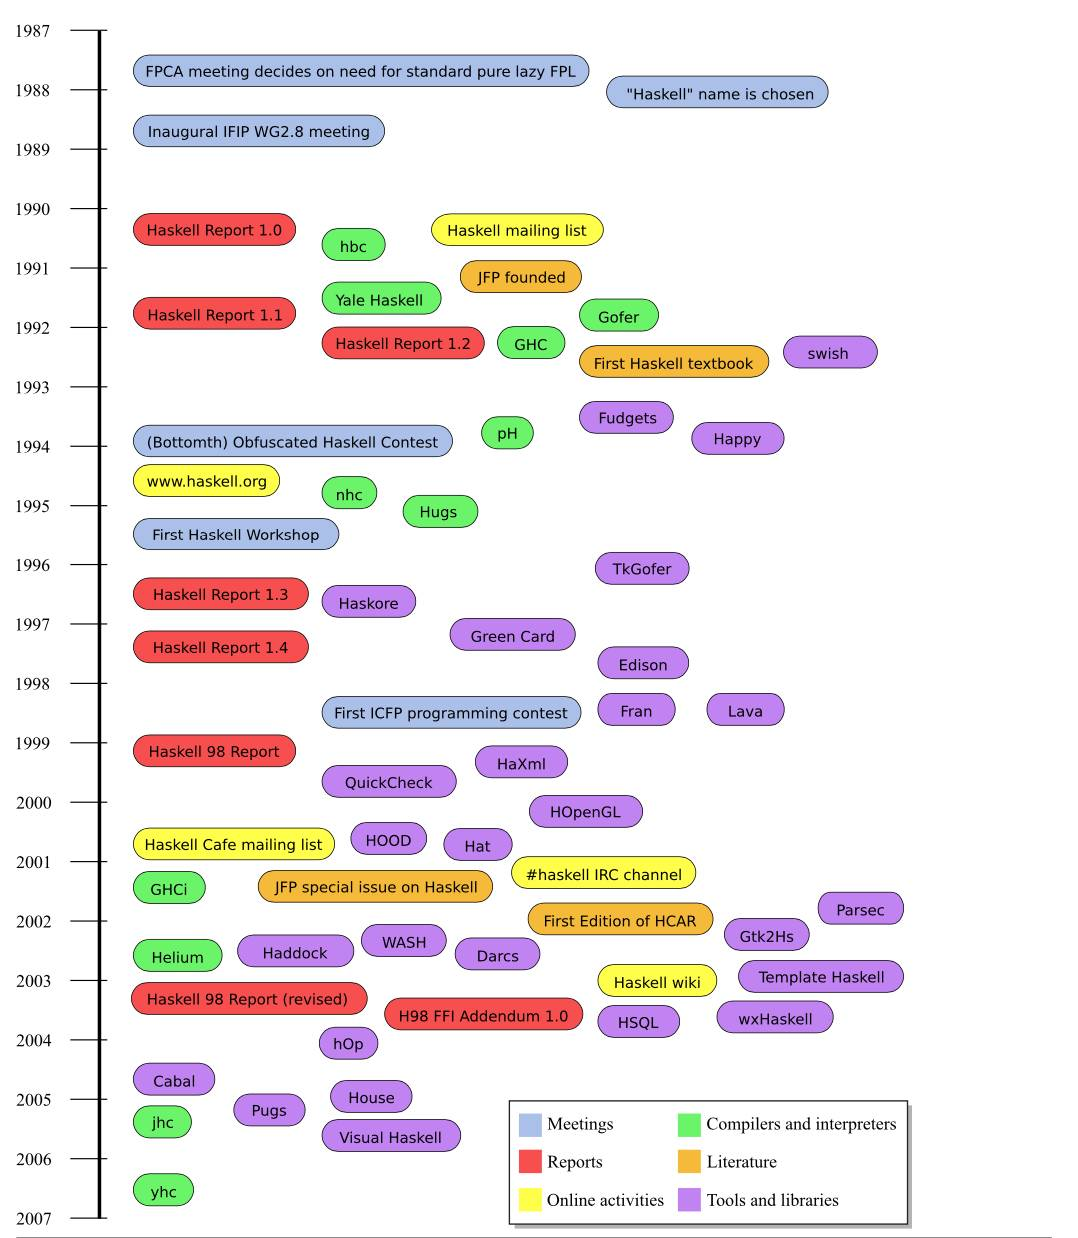
\includegraphics[width=.9\linewidth]{img/2023-05-18_12-50-04_screenshot.png}
\caption{A timeline of the history of Haskell, its creation and its development \autocite{hudakHistoryHaskellBeing2007}.}
\end{figure}

The first meeting was held at Yale during 1988. There, a clear list of Haskell's goals was defined (\hyperref[sec:org8322908]{Haskell's goals}) and a name was decided, that was although later changed (\hyperref[sec:org455326b]{Haskell's name}).

\subparagraph*{Haskell's name}
\label{sec:org455326b}

During the meeting, the members of the development team were encouraged to suggest names. The list included names such as ``Semla'', ``Vivaldi'', ``Mozart'', and more. After conversation each member was given the opportunity to mark a name they didn't prefer. Eventually, only one name remained, and it was decided that the language would be named after the mathematician Haskell B. Curry. Specifically the creators decided to keep the name of ``Haskell'' as the final name \autocite{hudakHistoryHaskellBeing2007}.

At first the chosen name was ``Curry''. But after a while, the committee came to the realization that they would have an overabundance of comical references regarding the name \autocite{hudakHistoryHaskellBeing2007}. Although there were various amusing jokes that could be made such as the spice carry, that is used in cooking, they were genuinely unsettled by the possibility of using Tim Curry as a way to make fun of the language.
As Jon Fairbairn's abstract machine was referred to as TIM and Tim Curry was well-known for his role in the \emph{``Rocky Horror Picture Show''}, they opted to steer clear of this direction. After additional deliberation the following day, they ultimately opted for the moniker ``Haskell'' for their novel programming language.

\subparagraph*{Haskell's goals}
\label{sec:org8322908}

At first the committee had to clearly set the purposes of the language. January 9th through 12th marked one very important gathering in which the following were decided \autocite{hudakHistoryHaskellBeing2007}:

\begin{enumerate}
\item The language should be appropriate for educating, doing inquiry, and lastly implementations, such as constructing big structures .

\item Analytic syntax and significations should be presented in order to provide the complete description of the language.

\item The language must be accessible to all, and everyone should have the freedom to utilize and share it without any restrictions.

\item It should be applicable as a foundation for additional language exploration and investigation.

\item The language's concepts should be founded upon commonly accepted ideas and principles.

\item The language should aim to minimize superfluous discrepancies among functional programming languages. To achieve this, the committee's preliminary decision was to derive it from an already established language, namely OL.
\end{enumerate}

The last two goals were proof that the original vision of Haskell was to rely on battle-tested methods and patterns and only unite the separated functional programming world. But this vision was short-lived, since neither OL was used as a base and Haskell introduced a myriad of new concepts in programming.

\paragraph*{The Haskell Report}
\label{sec:org4e66d36}

In a meeting of the committee in Glasgow during 1988, it was decided that Hudak and Wadler would be responsible for editing the \emph{first Haskell report}. This report would serve as a specification for the language. Its name was ``Report on the Programming Language Haskell, A Non-strict, Purely Functional Language''. It was finally published in April 1st of 1990, with version number 1.0.

Its next 1.1 revision was published in August of 1991 and 1.2 in March of the following year. 1.3 was published in 1996, with an added \emph{Library report}. 1.3 was the version which introduced \emph{monads} and monadic I/O. 1.4 was published in 1997, and two years after the \emph{Haskell 98 report} was released. This version was a big milestone for Haskell. It coincided with the disbandment of the Haskell committee. It was later revised and republished as a book in December of 2002, also being freely accessed online \autocite{hudakHistoryHaskellBeing2007}.

The latest Haskell report was published in 2010 and is considered the current definition of the Haskell language \autocite{marlowHaskell2010Language2010,haskellwikiHaskellHaskellWiki2023}.

\subsection{Haskell's popularity}
\label{sec:orgcb1b50b}

Haskell's popularity has been recorded by two major programming languages popularity indexes, the TIOBE and PYPL indexes \autocites{carbonnellePYPLPopularitYProgramming2023}[][]{tiobeTIOBEIndex2023}.

According to the TIOBE index, as of May of 2023 Haskell takes the 36th spot in programming language popularity \autocite{tiobeTIOBEIndex2023}. The TIOBE index is created and maintained by TIOBE Software BV, a company based in Eindhoven, the Netherlands. According to their \emph{About Us} page, they specialize in measuring code quality in software. The TIOBE index's ratings are based on the number of courses, jobs and users a given programming language has, and also many popular search engines such as Google and Bing.

The PYPL index ranks Haskell in the 28th spot, as of May of 2023 \autocite{carbonnellePYPLPopularitYProgramming2023}. Haskell's evolution in popularity from 2005 until today is shown in figure \ref{fig:org6a8e787}. The PYPL (PopularitY of Programming Language) index is based on the number of programming language specific tutorials are searched on Google \autocite{carbonnellePYPLPopularitYProgramming2023}.

Also of note is Haskell's subreddit\footnote{\url{https://www.reddit.com/r/haskell/}}, which according to \url{https://subredditstats.com/r/haskell} has around 74,500 subscribers and an all around upward trend.

\begin{figure}[htbp]
\centering
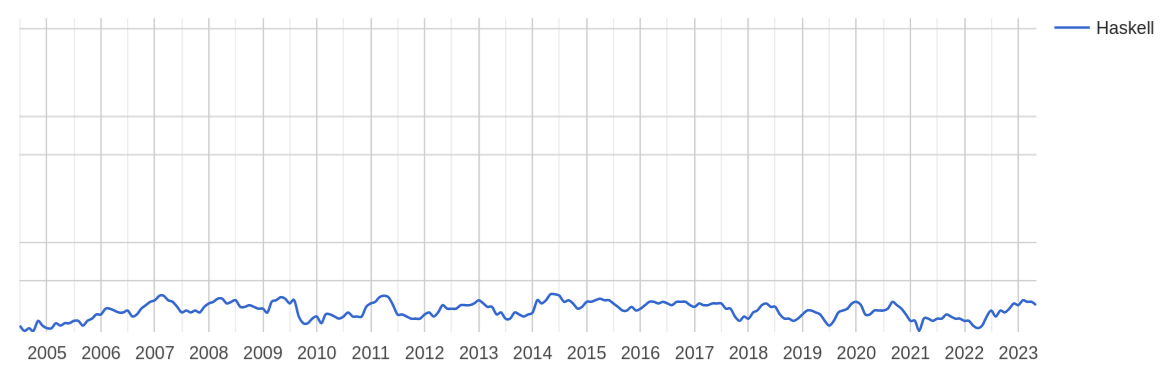
\includegraphics[width=.9\linewidth]{img/2023-05-18_17-15-08_screenshot.png}
\caption{\label{fig:org6a8e787}Haskell's worldwide popularity since 2005 in logarithmic scale \autocite{carbonnellePYPLPopularitYProgramming2023}}
\end{figure}

\subsection{Haskell's use cases}
\label{sec:orge06896e}

\subsubsection{Spam Filtering at Facebook}
\label{sec:org543ef8c}

Meta's secret weapon against spam and malware is a system called Sigma. Its job is to identify malicious actions on Facebook such as spam, phishing attacks, posting links to malware, etc. Threats detected by Sigma are removed automatically so they do not show up in the user's feed.

Meta recently completed a full redesign of Sigma, which involved replacing the in-house(custom) FXL language formerly used to power Sigma with Haskell. The Haskell-powered Sigma can now serve up to one million requests per second \autocite{marlowFightingSpamHaskell2015}. It is also important to note that the team behind Sigma's development also made several improvements to \texttt{ghc}, making it possible for Sigma to achieve better performance from Haskell compared to the previous implementation.

\paragraph*{How does Sigma work?}
\label{sec:orgf29b873}

Sigma is a rule engine, which means it runs a set of rules, called \emph{policies}. Every interaction on Facebook from posting a status update to clicking ``like'' results in Sigma evaluating this action with a set of policies specific to that type of action. These policies make it possible for Meta to identify and block malicious interactions.

\paragraph*{Why Haskell?}
\label{sec:org05d223e}

The original language that Meta designed for writing its policies, FXL, was not ideal for expressing the growing scale and complexity of Facebook policies. It lacked certain abstraction capabilities, such as user-defined data types and modules, and its implementation, based on an interpreter instead of a compiler, was rather slow. This is why they decided to migrate to an existing language \autocite{marlowFightingSpamHaskell2015}.

These are the features that were at the top of the team's list when choosing a replacement language:

\begin{enumerate}
\item Purely functional and strongly typed.

\item Automatic batching and ability to overlap of data fetches.

\item Push code changes to production in minutes. The fleet must get the
updated-compiled version of Sigma as fast as possible.

\item Performance.
\end{enumerate}

Haskell measured up quite well for the specific demands.

\subsubsection{Cardano}
\label{sec:org1a00c34}

Cardano is a blockchain platform that aspires to provide a secure and scalable infrastructure for creating decentralized applications and executing \emph{smart contracts}. It was founded by a group of researchers, engineers, and academics, including experts in functional programming languages like Haskell. The core software components of Cardano, including the blockchain protocol and smart contract infrastructure, are all written in Haskell \autocite{heisenbird-eokCharlesHoskinsonWhy2021}.

Haskell plays a key role in the development of Cardano, powering various aspects of its \emph{architecture} and \emph{functionality}. Here are some key areas where Haskell is utilized in Cardano:

\begin{itemize}
\item Blockchain Protocol: The central blockchain protocol, also known as \textbf{Ouroboros}, is a proof-of-stake (PoS) consensus algorithm that guarantees the security and integrity of the blockchain. Haskell's ability to specify complex protocols make it well-suited for implementing the \emph{consensus logic}.

\item Smart Contract Platform: The smart contract platform, called \textbf{Plutus}, allows developers to write smart contracts using functional programming techniques. Another popular choice for writing smart contracts is the Solidity language.

\item Daedalus Wallet: \textbf{Daedalus} is Cardano's official wallet. Daedalus provides users with a secure and user-friendly UI to manage their \textbf{ADA} (Cardano's native cryptocurrency) and use the blockchain.

\item Formal Verification: Haskell's support for formal methods and formal verification techniques. Formal methods involve mathematically proving the correctness of algorithms and protocols. Cardano wields formal methods to enhance its blockchain implementation.
\end{itemize}

Cardano benefits from the wide range of Haskell libraries and tools that are open-source. These libraries provide support for cryptography, networking, parsing, and other essential functionalities. The use of Haskell in Cardano reflects the language's suitability for building secure, high-assurance-availability systems.

\subsubsection{Hasura}
\label{sec:org2b21855}

Hasura is an open-source, real-time GraphQL engine that allows developers to quickly and easily build scalable, performant APIs for their applications \autocite{hasuraInstantGraphQLAPIs}. Developers can easily connect their databases to GraphQL, allowing them to access their data through a single API. Of course, it supports a variety of databases, including PostgreSQL, MySQL, Microsoft SQL Server, and Oracle. It provides a powerful set of features that make it easy to manage complex database schemas, including automatic schema stitching, real-time data synchronization, and granular access control.

One of the key benefits of using Hasura is its ability to generate a complete GraphQL API from an existing \textbf{database schema}. This means that developers can get up and running quickly without having to write any code, and they can easily update their APIs as their data schemas change over time. A rich set of tools for monitoring and debugging GraphQL APIs are provided, including query performance analysis and real-time tracing. It is highly customizable and extensible, with a large ecosystem of plugins and integrations that make it easy to integrate with other tools and services.

It has quickly become a popular choice for developers looking to leverage the power of GraphQL.

Haskell is a key component of Hasura's architecture. Hasura is built using Haskell, a language known for its strong type system, which helps catch errors at compile-time, and its support for lazy evaluation, which allows for efficient handling of large datasets. In general, Haskell is well-suited for building high-performance, scalable systems. For example, Hasura uses the Postgres database library for Haskell to provide seamless integration with a variety of databases.

\subsubsection{Hledger}
\label{sec:org952bcb7}

Hledger is a command-line tool for double-entry accounting, written in Haskell. It is part of the larger Plain Text Accounting paradigm\footnote{\url{https://plaintextaccounting.org/}}. It is cross platform. It can import from and export to various data formats such as CSV or TSV. Also, it has multiple choices for a User Interface: It can be used from the command-line, a web browser, on mobile, and has various editor/IDE plugins \autocite{michaelHledger2023}.

\subsubsection{Pandoc}
\label{sec:org899550d}

Pandoc is a Haskell library used for markup conversion. It is a powerful command-line tool that can inter-convert various file formats, e.g. DocX to PDF, \LaTeX{} to Markdown, Jupyter Notebook to HTML etc. An interesting feature is its Pandoc \emph{filters}, which can be written directly in Haskell and provide the ability to modify the intermediate Abstract Syntax Tree (AST) of the conversion \autocite{macfarlanePandoc2023}\footnote{Pandoc was also used extensively in the writing of this document for converting Markdown to Org-Mode, which was later exported to \LaTeX{} and then compiled to this PDF document.}.

\subsection{Tools and frameworks for developing in Haskell}
\label{sec:orgee64d32}

\subsubsection{Hackage}
\label{sec:org26a93c9}

Hackage is a key part of Haskell's ecosystem and provides a convenient way for Haskell developers to find and share code \autocite{hackageHackage2023}. Hackage is a central repository of open-source Haskell packages, similar to other package managers such as PyPi for Python or npm for JavaScript.

Hackage contains thousands of Haskell packages, each one provides a set of modules and functions that can be used in other projects. Packages are identified by a unique name and version number, and are organized into categories such as ``Web'', ``Database'', ``Parsing'', and so on. It provides a way to effortlessly download and install Haskell packages, including their dependencies. Developers can upload their own packages, making them available to everybody. Uploading a package to Hackage involves creating a Cabal (see \ref{sec:orgceb25dc}) file that describes the package and its dependencies, and then using Cabal to upload the package. Hackage uses a versioning system that allows multiple versions of a package to coexist. Thanks to the versioning system, developers can update their packages without breaking existing projects that depend on them.

\subsubsection{Haddock}
\label{sec:org1868b7c}

Haddock is a tool used for generating documentation from specially formatted comments in Haskell code \autocite{haddockHaddockDocumentation2023}. It is named after William Haddock, a British naval officer. Haddock markup is the syntax used for writing these comments, which is similar to HTML but specifically designed for documenting Haskell code. The generated documentation provides information about the functions, types, and modules defined in the code, as well as usage examples. The documentation can be generated in several formats, including HTML, \LaTeX{}, and Hoogle, a search engine for Haskell libraries.

Haddock is included in the Haskell Platform, a collection of tools and libraries for Haskell programming. It is also available as a standalone tool for use with other Haskell compilers and build systems.

Using Haddock for documentation is essential for ensuring that the codebase is well-documented and easily understandable. It helps to maintain code quality and encourages best practices in code development. Haddock is widely used in the Haskell community.

\subsubsection{HLint}
\label{sec:orgb33ce8c}

HLint is a useful tool for analyzing and optimizing Haskell code, designed by Neil Mitchell in 2006 \autocite{mitchellHLint2023}. It is an open-source project available under the BSD-3-Clause license. The main objective of HLint is to help Haskell developers write better code that is more efficient, readable, and maintainable. It achieves this by analyzing the code and identifying patterns that can be simplified or improved. Consequently it produces suggestions for refactoring the code, in order to enhance its quality and readability. Developers can use HLint to analyze individual Haskell files or complete projects. It can be easily integrated into their workflow by incorporating it with a range of tools, such as IDEs and text editors. Furthermore, it provides a web interface that can be used to search and browse through the suggestions offered. It also supports customizable rules and configurations that can cater to various coding styles and preferences.

\subsubsection{HUnit}
\label{sec:orga423afd}

HUnit is a unit testing framework and a key part of the broader Haskell ecosystem \autocite{HUnitUserGuide2023}. With HUnit, you can define test cases as functions that assert expected values against actual results. These test cases can be grouped together into test suites, which make it easy to organize and run multiple tests at once. HUnit provides a set of assertion functions that allow you to check conditions such as equality, inequality, and expected exceptions.

\begin{listing}[htbp]
\begin{minted}[]{haskell}
import Test.HUnit

-- Define the test cases
testAddition :: Test
testAddition = TestCase assertEqual "Addition test" 6 (2 + 4)

testSubtraction :: Test
testSubtraction = TestCase assertEqual "Subtraction test" 10 (30 - 20)

-- Create a test suite and include the test cases
tests :: Test
tests = TestList [testAddition, testSubtraction]

-- Run the tests using the runTestTT function
main :: IO ()
main = runTestTT tests
\end{minted}
\caption{\label{lst:orga7c7406}Simple example of a test case using HUnit}
\end{listing}

In listing \ref{lst:orga7c7406}, \texttt{testAddition} is a test case that asserts the expected value 6 against the result of the addition 2 + 4. The \texttt{assertEqual} function is used to perform the equality check. As you can see, the \texttt{testSubtraction} test case performs a similar check. The \texttt{tests} function defines a test suite that includes the \texttt{testAddition} and \texttt{testSubtraction} test cases. Finally, the main function runs the tests using the \texttt{runTestTT} function, which prints the results to the console.

By leveraging HUnit, Haskell developers can automate the testing process and easily detect bugs and errors in their code. Unit tests help ensure the reliability and correctness of software, providing confidence.

\subsubsection{QuickCheck}
\label{sec:orgf82d963}

QuickCheck is a library for automated testing of Haskell programs \autocite{claessenQuickCheckAutomaticTesting}. It was developed by Koen Claessen and John Hughes and is based upon the concept of property-based testing. Traditional testing involves writing test cases that check for expected outputs given specific inputs. In contrast, QuickCheck focuses on defining properties that must always hold true for your program, the input. It then generates random inputs and checks that these properties hold true for each one. For example, if you're testing a function that sorts a list of integers, you could define a property like ``sorting a list should produce a list in ascending order''. QuickCheck will generate random lists of integers and check that this property holds for each one.

To use QuickCheck, you define properties using the property function, which takes a \texttt{Boolean} expression that should hold true for all possible inputs. You can also use generators to define the types of inputs that it will generate. For instance, you can define a generator for lists of integers or for strings. Once you have defined your properties and generators, you can run it using the quickCheck function. QuickCheck will report any failures and reduce input values to find the minimal counterexample.

QuickCheck is a powerful testing tool that can help you find bugs and edge cases that you might miss with traditional testing. By generating random inputs, it can help you test your program more thoroughly and find unexpected issues that you may not have considered. It's a great addition to any Haskell developer's testing toolkit.

\subsubsection{Yesod}
\label{sec:org3bf311e}

Yesod is a powerful and flexible web framework for Haskell that is designed to be high-level, type-safe, and scalable \autocite{yesodYesodWebFramework2023}. It provides a powerful set of tools and abstractions for building web applications. It also provides a type-safe DSL (Domain-specific language) for defining routes in your application. With its help you can be sure (at compile-time) that the URLs of your application are valid and that the provided parameters are correct. There is an ORM (Object-Relational Mapping) library included called \textbf{Persistent}, which allows you to interact with a database in a type-safe and composable way. Persistent supports several different database backends, including PostgreSQL, MySQL, and SQLite.

Yesod has a type-safe library for defining and rendering HTML. Additionally, it has built-in support for user authentication and session management. Its libraries support automatic validation, error reporting, password hashing, CSRF protection, and other security-related tasks.

\subsubsection{Happy \emph{and} Alex}
\label{sec:orge83fedb}

Happy and Alex are two popular tools used in Haskell programming for generating parsers and lexers respectively. They greatly simplify the process of handling complex input formats by automatically generating the necessary code based on provided specifications of a grammar.

They are two different tools that are usually used together. Happy, also known as the Happy Parser Generator, is designed for generating parsers in Haskell \autocite{Happy2023}. It takes a specification file and generates a Haskell module able to parse input according to the specified grammar. Happy has support for both LALR(1) and GLR parsing algorithms, providing flexibility in handling different grammatical constructs. Additionally, it allows programmers to specify semantic actions to be executed during the parsing process, enabling the manipulation and interpretation of parsed data.

Alex, or the Alex Lexer Generator, is used for generating lexical analyzers in Haskell \autocite{AlexLexicalAnalyser2023}. It takes a specification file containing regular expressions and associated actions and generates a Haskell module able to perform lexical analysis on input text. Alex employs efficient algorithms, such as finite automata and lazy evaluation, to generate high-performance lexers. Lexical analysis amounts to breaking the input into tokens, which are subsequently consumed by a parser generated by Happy.

By separating the concerns of parsing and lexing from the rest of the code, Happy and Alex allow developers to focus on the core logic of their programs. They automate the generation of code that can handle complex input structures, saving developers time and effort. Moreover, the generated parsers and lexers are highly optimized, contributing to the overall performance of the Haskell programs.

\subsubsection{Cabal}
\label{sec:orgceb25dc}

Cabal is a build system and package manager for Haskell \autocite{Cabal2023}. It provides a way to manage dependencies and build Haskell projects, making it easier to develop and distribute Haskell software. In Cabal, a package is a collection of Haskell \emph{modules} and other files that can be compiled into a library or executable. Each package is identified by a unique name and version number. Dependencies are declared in a package's Cabal file, which lists the names and version ranges of the required packages. There is a build system that can compile Haskell code into executables and libraries. It uses the GHC compiler by default, but can also work with other compilers such as Hugs or JHC. Cabal also integrates with Hackage (see \ref{sec:org26a93c9}), the central repository of open-source Haskell packages.

Cabal supports sandboxing, which allows you to create isolated environments for your projects. This can be useful for testing and development, since it ensures that dependencies are not shared between projects and avoids version conflicts. It is similar to Anaconda for Python.

Cabal is widely used in the Haskell community and is a key part of the Haskell development toolchain.

\subsubsection{The Haskell Tool Stack (Stack)}
\label{sec:org5e53684}

Stack is a popular build tool for Haskell that was originally created to solve problems that developers were facing with Cabal (see \ref{sec:orgceb25dc}), another Haskell build tool \autocite{CommercialhaskellStack2023}.

The main focus of Stack's design point is reproducible builds. If you run \texttt{stack build} today, you must get the same result as running \texttt{stack build} tomorrow. To simplify this process, Stack uses curated package sets called snapshots.

One of the biggest advantages of Stack is that it provides deterministic builds. This means that if you build your project with Stack, you should get the same results every time, regardless of the environment you're building in. This makes it easier to reproduce builds across different machines and ensure that your code is consistent. Stack manages dependencies using snapshots, which are collections of packages that have been tested together and are sure to work together. This means that the dependencies you're using are compatible with each other, reducing the risk of conflicts. It is important to note that Stack has built-in support for caching compiled packages and dependencies. Stack supports multi-package projects. This can be useful if you're working on a large project that is split into multiple packages.

Stack is relatively easy to set up and use. It is easy to get started with a new project using the \texttt{stack new <project-name>} command. Finally, Stack integrates well with other Haskell tools such as Haddock and GHCi.

\section{Analyzing Haskell}
\label{sec:org84207c6}

\subsection{Control Structures}
\label{sec:org85fe324}

Usually functional languages like Haskell do not have constructs to change the execution path or to provide loops. Languages of this category try to follow mathematical notation for function definition and as a result they provide multiple definitions of the same function to cover different input cases. This approach requires that the language has pattern matching capabilities. However, some functional languages like Haskell provide some control constructs to facilitate programmers' work.

\subsubsection{Pattern Matching}
\label{sec:orgc0cc741}

Pattern matching is a mechanism used to distinguish a structure of variables and constructors (either predefined or user-defined), called \emph{pattern} \autocite[chapter 3.17]{marlowHaskell2010Language2010}.

A given value fulfills a pattern if there is a substitution of its variables so that the instantiated pattern evaluates to the given value. Pattern matching can be used to provide multiple definitions of a function or within a case expression

\paragraph*{Case Expression}
\label{sec:orge8accdf}

In Haskell, the \texttt{case} expression is a control structure used for pattern matching and branching based on the structure of a value. It helps the language to handle pattern matching of complex expressions or to express multiple possible outcomes in a single expression \autocite{kremerCPSC449Programming2015}.

The syntax for the \texttt{case} clause is shown in listing \ref{lst:org725b230}, and in listing \ref{lst:org336e917} the \texttt{if-then-else} clause implemented with \texttt{case} is shown.

\begin{listing}[htbp]
\begin{minted}[]{haskell}
case expression of
    pattern1 -> result1
    pattern2 -> result2
    ...
    patternN -> resultN
\end{minted}
\caption{\label{lst:org725b230}\texttt{case} clause}
\end{listing}

\begin{listing}[htbp]
\begin{minted}[]{haskell}
case expression of
    True  -> result1
    False -> result2
\end{minted}
\caption{\label{lst:org336e917}\texttt{if-then-else} clause using \texttt{case}}
\end{listing}

\subsubsection{Guards}
\label{sec:orgae8ba1b}

Guards is a control construct that is used to specify conditions to be satisfied for a portion of a program. Guards are typically used with function declarations as follows and they are represented by a pipe (\texttt{|}) \autocite{kremerCPSC449Programming2015}. An example is shown in listing \ref{lst:org1409821} (\texttt{otherwise} is just an alias to \texttt{True}).

\begin{listing}[htbp]
\begin{minted}[]{haskell}
factorial :: Int -> Int
factorial n
    | n < 0     = error "Given number: negative -> factorial: undefined."
    | n == 0    = 1
    | otherwise = n * factorial (n - 1)
\end{minted}
\caption{\label{lst:org1409821}Example of a function declaration using guards}
\end{listing}

\subsubsection{Monads}
\label{sec:org5703e2d}

\paragraph*{Definition}
\label{sec:org6dd58e9}

A \emph{Monad} is a subclass of Applicative class that is defined by the following three things \autocite{wikibooksHaskellUnderstandingMonads2021}:

\begin{enumerate}
\item A type constructor
\item A return function
\item A ``bind'' operator (\texttt{>{}>{}=}).
\end{enumerate}

\begin{listing}[htbp]
\begin{minted}[]{haskell}
class Monad m where
    (>>=)  :: m a -> (a -> m b) -> m b
    (>>)   :: m a -> m b -> m b
    return :: a -> m a
    fail   :: String -> m a
    
    m >> k = m >>= \_ -> k
    fail s = error s
\end{minted}
\caption{Monad class according to Haskell 2010 Language Report \autocite[chapter 6.3.6]{marlowHaskell2010Language2010}}
\end{listing}

\begin{listing}[htbp]
\begin{minted}[]{haskell}
class (Functor f) => Applicative f where
    pure  :: a -> f a
    (<*>) :: f (a -> b) -> f a -> f b
\end{minted}
\caption{Applicative class \autocite[chapter 29.1.1]{wikibooksHaskellWikibooksFree2022}}
\end{listing}

Monads provide a way to handle effects and control flow in a pure functional language like Haskell. Monads facilitates the encapsulation of computations that involve side effects or non-determinism and give the ability to control their sequencing and interaction.

\paragraph*{\texttt{do} Notation}
\label{sec:org03da3d5}

\begin{listing}[htbp]
\begin{minted}[]{haskell}
do
  statement1
  statement2
  ...
  statementN
\end{minted}
\caption{General syntax of \texttt{do} notation}
\end{listing}

The usage of \texttt{do} expressions is a convenient way to compose monadic action in Haskell and gives the user the ability to write imperative-like code inside a monad (e.g. I/O monad). Furthermore, \texttt{do} expressions make the code more readable and as a result maintainable by making the sequence of actions and the handling of produced results simpler \autocite{kremerCPSC449Programming2015}.

\begin{listing}[htbp]
\begin{minted}[]{haskell}
sumTwoNumbers :: IO ()
sumTwoNumbers = do
  putStrLn("Enter a number: ")
  num1 <- readLn
  putStrLn("Enter a second number: ")
  num2 <- readLn
  let result = num1 + num2
  putStrLn ("The sum of the 2 given numbers is: " ++ show result)
\end{minted}
\caption{Haskell program to sum 2 numbers using do notation \autocite[chapter 10.2]{wikibooksHaskellWikibooksFree2022}}
\end{listing}

\subsubsection{Recursion}
\label{sec:org08741b5}

Haskell does not have a control structure to achieve repetition. This feature is provided using recursion, which makes it a fundamental and very powerful tool for working with lists and other similar structures. The repetition is achieved using recursive functions that call themselves with modified arguments, until they reach the defined base case \autocite{kremerCPSC449Programming2015}.

\begin{listing}[htbp]
\begin{minted}[]{haskell}
factorial :: Int -> Int
factorial 0 = 1
factorial n = n * factorial (n - 1)
\end{minted}
\caption{Haskell program to find the factorial of a number using recursion}
\end{listing}

\subsection{Laziness}
\label{sec:org18a698d}

Lazy evaluation is an evaluation approach that postpones the computation of a statement until the value of it is wanted. This has as the following result: The evaluation doesn't spend more time for excessive and useless calculations. This feature caught the attention of many experts. Many scientists gathered in order to contribute to the design of the language.

In Haskell, expressions in this context are not assessed when connected to variables. Instead, their evaluation is postponed until the results are necessary for other calculations. As a result, arguments are not assessed before being passed to a function. Their evaluation only takes place when their values are actually utilized. This method is known as \emph{call by name} \autocite{haskellwikiHaskellHaskellWiki2023}.

Although lazy evaluation offers numerous benefits, its primary disadvantage lies in the unpredictability of the usage of the memory. The challenge arises because expressions such as \mintinline{haskell}{5+5 :: Int} and \mintinline{haskell}{10 :: Int} --- which produce the same value of 10 --- may not have the same sizes, resulting in problems with the memory such as irregular memory usage.

\subsubsection{Lazy evaluation and semantics}
\label{sec:org3a9ac74}

Operational semantics in Haskell define how a program is examined, and lazy evaluation is a key aspect of it. Conversely, denotational semantics includes non-strict semantics, which describe what a program calculates. The non-strict semantics approach enables the handling of values that are not defined, and also permits the processing of unending data.

\subsection{Identifiers}
\label{sec:orgf2005e2}

\begin{figure}[htbp]
\centering
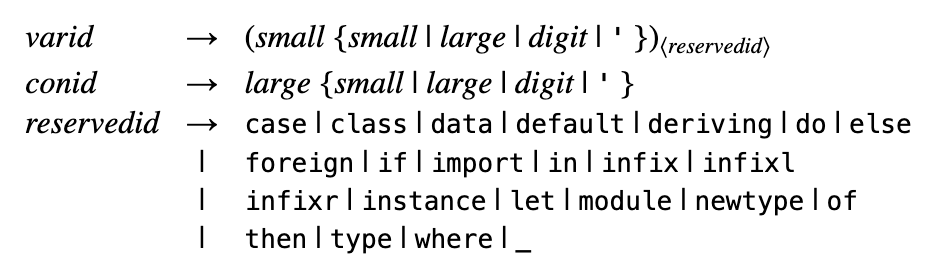
\includegraphics[width=.9\linewidth]{img/2023-05-22_21-55-01_screenshot.png}
\caption{Identifiers in BNF notation \autocite[section 2.4]{marlowHaskell2010Language2010}}
\end{figure}


\subsubsection{Rules}
\label{sec:orgd565d08}

Identifiers in Haskell start by a letter that can be followed by any combination of zero or more letters, digits, quotes or underscores. Underscore by itself is a reserved identifier and in patterns can act as a wildcard. Identifiers are also case sensitive and keywords such as if, infix, else etc cannot be used as identifiers.

\subsubsection{Purpose}
\label{sec:orge1bf1cd}

Identifiers are used to name program entities in Haskell programs. These entities contain variables, functions and data types. Every used identifier must obey the same strict name restrictions and they would better follow some naming conventions that will be described later. Worth mentioning that Haskell is a statically typed language which means that the type of an identifier is determined at compile time.

\subsubsection{Scope}
\label{sec:org9fc9519}

The scope of an identifier indicates the part of the program that can access it. In Haskell there are 3 possible scopes for each identifier:

\begin{itemize}
\item Global scope: The identifiers that are declared at the top level of the module can be accessed by the entire module.

\item Local scope: The identifiers that are declared in a block of code can only be accessed within this block. Every use of them outside the specific block is invalid.

\item Parameter scope: The identifiers that are declared as parameters of a function can only be accessed within this specific function.
\end{itemize}

\subsubsection{Naming conventions}
\label{sec:orgdf7c566}

The name of an identifier is important to be meaningful and descriptive so the code gets more readable, understandable and maintainable. Also, a good practice is to follow the following conventions \autocite{haskellwikiProgrammingGuidelinesHaskellWiki2022}:

\begin{itemize}
\item Type names should start with capital whereas function names with a lowercase letter, so only avoid infix identifiers.

\item Laconic and descriptive names are preferred but if longer names are needed they should be in \texttt{lowerCamelCase}.

\item Type, type class, and constructor names should be written using \texttt{UpperCamelCase}.

\item In the standard libraries, some parts of the code are written in \texttt{snake\_case} for long identifiers to better reflect names given with hyphens in the required documentation. Such names should be transliterated to \texttt{camelCase} identifiers if they get used out of the libraries by possibly adding a suffix or prefix to avoid conflicts with keywords.
\end{itemize}

\subsection{Keywords}
\label{sec:orgec88207}

\subsubsection{\texttt{data}}
\label{sec:org6f2a4ae}

The keyword \texttt{data} is often used in many cases. One very popular case is the creation of an algebraic data type. These kind of data types involve the combination of types through many different ways. The result is the creation of complex types. An example of it's use can be the following:

\begin{minted}[]{haskell}
data Mammal a = Cat a
              | Animal (Mammal a) (Mammal a)
\end{minted}

\subsubsection{\texttt{data family}}
\label{sec:org5cfa9b0}

Type families offer a method to declare functions. The environment they are created in is called type level. These functions can be used to connect different presentations. This way a more polymorphic type system can be accomplished. Specifically, data families illustrate data and newtype declarations in a method which is indexed. For example, the definition of a data family in the form of list is:

\begin{minted}[]{haskell}
data family ANOTHERLIST l
\end{minted}

\subsubsection{\texttt{data instance}}
\label{sec:orgc4a7169}

This keyword relates to paragraph \hyperref[sec:org5cfa9b0]{\texttt{data family}}. Specifically, they enable the declaration of types. So this keyword offers a guide for the execution of the above types.

\subsubsection{\texttt{default}}
\label{sec:org1159fa3}

In Haskell many obscurities can happen when using the class \texttt{Num}, so a way of handling them is by using the \texttt{default} declaration.

\subsubsection{\texttt{deriving}}
\label{sec:org14f3506}

This keyword provides an automatic creation of often used actions for data types that are declared from the user. For example a data type can be defined as an instance of the \texttt{Show} class. This derived instance for \texttt{Show} provides an automatic creation of the \texttt{show} operation. The \texttt{show} operation transforms a value of the data type into a string illustration.

\begin{minted}[]{haskell}
data Action = Temp
            deriving (Eq)
\end{minted}

\subsubsection{\texttt{deriving instance}}
\label{sec:org8a8c171}

It is used in order to define an instance. It refers to a type class. These are created for data types that already exist. They are created differently from the data type. For example:

\begin{minted}[]{haskell}
data MyType = MyType Int
deriving instance Show MyType
\end{minted}

So from the above commands, instances of \texttt{MyType} can be printed with the below commands.

\begin{listing}[H]
\begin{minted}[]{haskell}
myValue = MyType 35
print (show myValue)
\end{minted}
\caption{When this code block executes, the result will be: ``MyType 35''}
\end{listing}

\subsubsection{\texttt{do}}
\label{sec:org228107d}

This keyword offers an easier way of using monads. Using the \texttt{do} notation the creation of code that specifies authoritative programming is possible. For example we have the following:

\begin{minted}[]{haskell}
do {a ; b <- c ; process b}
\end{minted}

In the above example \texttt{a} illustrates an operation that is executed but its output is not assigned to a variable. Also \mintinline{haskell}{b <- c} is a way of binding that retrieves the value from the monadic computation \texttt{c} and binds it with \texttt{b}.

\subsubsection{\texttt{forall}}
\label{sec:orga51dd04}

In Haskell, type variables are considered universally assessed (by default). This means that there's no need for the type variables to be quantified universally. However it is very often in Haskell that a programmer wants to clarify the quantification distinctly. So the \texttt{forall} keyword is used in order to achieve that. For example the following syntax:

\begin{minted}[]{haskell}
forall b.b -> b
\end{minted}

\subsubsection{\texttt{foreign}}
\label{sec:org9cf5244}

This keyword is useful in case a programmer wants to use a function that it is not defined in any Haskell's library or to give permission to another language to use functions that are written in Haskell. The most common commands are \mintinline{haskell}{foreign import declaration}, and \mintinline{haskell}{foreign export declaration}. The first one gives permission to a programmer that writes a program in Haskell to use a function which is not included in any Haskell library. The second gives permission to non Haskell programming languages to use a function which is created in Haskell.

\subsubsection{\texttt{hiding}}
\label{sec:orgf808421}

Haskell allows to include a module and avoid the entities that are useless. The keyword \texttt{hiding} handles entities that are useless for the program. Specifically, it excludes them keeping for the program only entities that are useful. The syntax is the following: \mintinline{haskell}{import Data.List hiding (sort, isInfixOf, intersperse)}.

\subsubsection{\texttt{if}, \texttt{then}, \texttt{else}}
\label{sec:orgbce238e}

Haskell --- just like other programming languages --- offer a way to create conditional expressions. A program evaluating a condition has some options in order to choose between expressions. The syntax is the following:

\begin{minted}[]{haskell}
if condition then expression1 else expression2
\end{minted}

\subsubsection{\texttt{import}}
\label{sec:org3293fe0}

In Haskell the reference between modules is possible. This can happen with the keyword \texttt{import}. This way modules can use entities that belong to other modules. The general form of the keyword is: \mintinline{haskell}{import ModuleName (entity1, entity2, ...)}.

\subsubsection{\texttt{infix}, \texttt{infixl}, \texttt{infixr}}
\label{sec:org0d26960}

Fixity declaration is a feature which is used to declare the method that the operators can be associated and the priority which they tie in expressions. It gives the ability of defining the behavior of operators when they appear together. These are the following kind of fixity declarations:

\begin{enumerate}
\item Infix left-associative

\item Infix right-associative

\item Infix non-associative
\end{enumerate}

The higher the number the higher the priority of evaluating the operator first in an expression. For example: \mintinline{haskell}{infixl 6 +}. This state says that addition has left-associativity and the precedence of it is 6.

\subsubsection{\texttt{instance}}
\label{sec:org7e4610e}

A type can be defined as an instance. It will refer to a class. This method is done using this keyword. Also it allows to provide the implementations for the class methods that are associated with it.

\begin{minted}[]{haskell}
instance ClassName Type where
\end{minted}

\subsubsection{\texttt{let}, \texttt{in}}
\label{sec:org4aca8e2}

These keywords are commonly used in order to define variables in a specific scope. If the \texttt{in} keyword is included then it states the scope of the declaration, else the declaration is considered as district. Finally the syntax is the following:

\begin{minted}[]{haskell}
let declaration1 ; ... ; declarationn in s
\end{minted}

\subsubsection{\texttt{module}}
\label{sec:orga724e59}

It's a container that holds related definitions, functions, types, entities etc.

\subsubsection{\texttt{newtype}}
\label{sec:org6adaf2b}

This keyword is used as a way to create new types. Specifically those types are the existing algebraic data types, but with different names. This method offers a way to present distinct types that have the same representation as existing ones. The syntax is

\begin{minted}[]{haskell}
newtype NewTypeName = Constructor ExistingType
\end{minted}

The difference between \texttt{newtype} and other type declaration keywords is that it forces stricter type-checking.

\subsubsection{\texttt{proc}}
\label{sec:orgb96e7b2}

The keyword \texttt{proc} is responsible for the definition of a very important feature. It is called \emph{arrow abstractions}. The result of it is the creation of an arrow. An arrow is a generalized function. It is used because of it's expressiveness when it comes to illustrating calculations and control flow. The syntax of this keyword is the following:

\begin{minted}[]{haskell}
proc pattern -> do
-- Arrow computations
\end{minted}

\subsubsection{\texttt{qualified}}
\label{sec:org5a7a3e9}

The keyword \texttt{qualified} is used as a way to include a module. However in this case the presentation of its name inside the scope can be avoided. This technique is often used when there are entities of modules with the same names, so the danger of a conflict happening is high. For example:

\begin{minted}[]{haskell}
import qualified Data.Text
\end{minted}

\subsubsection{\texttt{rec}}
\label{sec:orgc51f4d1}

This keyword is used in conjunction with a specific flag (\texttt{-XDoRec}). It is used in order to activate connections. Those connections have recursion. This occurs within the \texttt{do} block. By default this is not allowed. A \texttt{do} block is a way of putting in order operations.

\subsubsection{\texttt{type}}
\label{sec:org55c9389}

\texttt{type} can be used as a way of renaming an already existing algebraic data type, and every time this type is referred within the program with the new name it is being executed. This way, it is more convenient to refer to complex types. For example \mintinline{haskell}{type PhoneNumber = String}.

This way, whenever a program uses the type \texttt{String} it can use the type \texttt{PhoneNumber} (which are the same now) as well and if there's a reference of type \texttt{PhoneNumber} it can be used wherever the original type (\texttt{String}) is anticipated.

\subsubsection{\texttt{type family}}
\label{sec:org6306a60}

In Haskell a \texttt{type family} enables type generalization. It is used as a way to declare specific types (family types). They are synonyms and they are related.

\subsubsection{\texttt{type instance}}
\label{sec:org9d163ee}

This keyword is used in order to create an instance of the above kind of type.

\subsubsection{\texttt{where}}
\label{sec:org07e7497}

It allows to declare a definition, like a function or a value, that can be seen and used inside a scope. The \texttt{where} statement is attached to some construct like a function definition and can be used in relation to that. For example:

\begin{minted}[]{haskell}
calculateDiscount :: Double -> Double -> Double
calculateDiscount price discountRate = discountedPrice
  where
    discountedPrice = price - (price * discountRate)
\end{minted}

The \texttt{where} statements declare the variable within the where clause, we define \texttt{discountedPrice}, which in this case illustrates the price after the discount.

\subsubsection{\texttt{\{} and \texttt{\}}}
\label{sec:org6192557}

This keyword is used in order to define the scope of various statements. The statements are separated from each other with a semicolon (\texttt{;}). For example:

\begin{minted}[]{haskell}
doSomething = { x = 10; y = 20; z = x + y }
\end{minted}

Also this keyword is used in records. For example:

\begin{minted}[]{haskell}
record field1 = value1, field2 = value2, ...
\end{minted}

\subsubsection{\texttt{\{-} and \texttt{-\}}}
\label{sec:orge877ae7}

This is used as a way to write multi-line comments in Haskell. Specifically everything inside the \texttt{\{-} and \texttt{-\}} is considered as a comment and will be avoided from the compiler during the compilation.

\subsubsection{\texttt{|}}
\label{sec:org4252349}

A pipe can be used in the following cases:


\begin{enumerate}
\item This keyword is used to divide various constructors inside a data type definition. Each one illustrates a value that the data type can take. For example:

\begin{minted}[]{haskell}
   data Result a = Success a
                 | Failure String
\end{minted}

\item It is used in lists. For example:

\begin{minted}[]{haskell}
   positiveSquares = [a + a | a -> [2..], a > 0]
\end{minted}

\item It is used in order to separate conditions or guards in a function definition. For example:

\begin{minted}[]{haskell}
   isPositive :: Int -> Bool
   isPositive x
     | x > 0 = True
     |otherwise = False
\end{minted}
\end{enumerate}

\subsubsection{\texttt{\textasciitilde{}}}
\label{sec:org1adbdb4}

The tilde is used in order to denote a lazy pattern bind. They provide a mechanism for introducing patterns that are evaluated when needed. This type of behavior can be particularly useful when dealing with possibly infinite data structures.

\subsubsection{\texttt{`}}
\label{sec:orge239026}

This feature allows to use infix notation inside statements \autocite{marlowHaskell2010Language2010}. For example backticks can be used to treat add as an infix operator: \mintinline{haskell}{result = 5 `add` 3}.

\subsubsection{\texttt{\_}}
\label{sec:orgf243a1d}

It is used as a token that matches a value. It basically represents a value that there's no need to distinctly name. For example:

\begin{minted}[]{haskell}
getFirstElement :: [a] -> Maybe a
getFirstElement [] = Nothing
getFirstElement (x:_) = Just x
\end{minted}

\subsubsection{\texttt{\textbackslash{}}}
\label{sec:org2454627}

The backlash is used as a way to split a string in many lines. For example:

\begin{minted}[]{haskell}
s = "hi\
    hello"
\end{minted}

It is also used as a way to define anonymous functions. For example:

\begin{minted}[]{haskell}
subtract = \x -> x - 1
\end{minted}

\subsubsection{\texttt{[|} and \texttt{|]}}
\label{sec:org75fa73c}

It is used in the following cases:

\begin{enumerate}
\item It allows the treatment of the quoted expression as a first-class value.

\item To illustrate a declaration.

\item To illustrate a type.

\item To illustrate a pattern.

\item To define a quoting syntax.
\end{enumerate}

\subsubsection{\texttt{@}}
\label{sec:orgff2b71b}

It offers a method to give a name to a sub-pattern. This allows to refer to the matched value by the given name in the scope. For example:

\begin{minted}[]{haskell}
example :: [Int] -> [Int]
example inputList = case inputList of
newList@(first:remaining) -> if first == 0 then
remaining else newList
\end{minted}

The pattern \mintinline{haskell}{newList@(first:remaining)} is an as-pattern. It matches the list if it starts with an element first followed by the remaining elements remaining. The matched list is assigned the name \texttt{newList}.


\subsubsection{\texttt{*}}
\label{sec:org6a75cf9}

In Haskell the form of specific types (boxed) are represented with the symbol \texttt{*}. For example the \texttt{*} kind indicates that Int is a boxed type.

\subsubsection{\texttt{?}}
\label{sec:org5c75693}

It is used in cases like the following:

\begin{minted}[]{haskell}
ghci> :t ?name ++ " is awesome!"
  ?name ++ " is awesome!" ::
  (?name :: String) => String
\end{minted}

In this example, \texttt{?name} is an implicit parameter of type \texttt{String}. The expression \mintinline{haskell}{?name ++ " is awesome!"} concatenates the value of \texttt{?name} with the string `` is awesome!''.

\subsubsection{\texttt{=>}}
\label{sec:org0ae05cf}

It is used to specify constraints on the type variables or type classes that are involved in the function signature.

\subsubsection{\texttt{<-}}
\label{sec:orgea67499}

\begin{enumerate}
\item It is used to bind the result of a monadic action to a variable.

\item It is used in lists.

\item It is used to match a pattern and connect values in a guard.
\end{enumerate}

\subsubsection{\texttt{;}}
\label{sec:org97ea029}

It is used as a way to divide expressions in a sequence of statements that are enclosed in braces. For example:

\begin{minted}[]{haskell}
do {
putStrLn "Hello";
putStrLn "World";
}
\end{minted}

\subsubsection{\texttt{::}}
\label{sec:orga963f3f}

It is used to indicate the type signature of a declaration. For example:

\begin{minted}[]{haskell}
add :: Int -> Int -> Int
\end{minted}

The \texttt{::} operator specifies the type signature of the function, indicating that add has the type:

\begin{minted}[]{haskell}
type [Int] -> Int -> Int
\end{minted}

\subsubsection{\texttt{->}}
\label{sec:orged5e0b1}

\begin{enumerate}
\item It is used to denote the type of a function that takes one or more arguments and returns a result.

\item They are used in functions (lambda).

\item It is used in case expressions.

\item It is used in a specific feature (view patterns) that allows pattern matching

\item It is used in a specific feature (functional dependencies).
\end{enumerate}

\subsubsection{\texttt{-<{}<{}}}
\label{sec:org5fed568}

It is used as a way to express calculations in a way that uses arrows.

\subsubsection{\texttt{!}}
\label{sec:orgce22839}

Algebraic datatypes in Haskell are defined by constructors, which take one or more arguments. When a new value is created using a constructor, the corresponding values that will be merged to create the final value are generated by evaluating the arguments.

Haskell follows lazy evaluation by default, implying that the arguments supplied to a data constructor are not computed until they are required. This approach can be inefficient at times, especially when the arguments are either \emph{pricey} to calculate or not utilized at all.

Haskell handles this by giving the permission for the definition of strictness for the arguments that were offered to a constructor. In these cases with the use of a strictness flag represented by the symbol \texttt{!}, which is included in the algebraic datatype declaration. They are used in order to specify the arguments that must be calculated immediately upon constructor implementation \autocite{marlowHaskell2010Language2010,haskellwikiHaskellHaskellWiki2023}.

If the goal is the definition of a binary tree data type in Haskell, we can depict a binary tree as a node containing a value and two children, where each child can either be another node or an empty leaf. We can establish this data type using two constructors; one for the internal nodes and another for the leaves (listing \ref{lst:org226d47f}).

\begin{listing}[htbp]
\begin{minted}[]{haskell}
data BinaryTree a = Node a !(BinaryTree a) !(BinaryTree a)
  | Leaf
\end{minted}
\caption{\label{lst:org226d47f}Definition of the \texttt{BinaryTree} datatype.}
\end{listing}

The \texttt{BinaryTree} data type, consisting of two constructors: \texttt{Node} and \texttt{Leaf}. The \texttt{Node} constructor receives three arguments - a value of type ``a'', and two \texttt{BinaryTree} ``a'' values that represent the node's left and right children. The presence of an exclamation point before each child argument specifies that the children must be strictly evaluated. This denotes that their values will be calculated before the \texttt{Node} constructor is utilized, ensuring that the entire \texttt{BinaryTree} value is wholly computed during its construction.

Also, the exclamation point is further utilized denoting rigor within patterns (see listing \ref{lst:org0ec0035}). The function uses a bang pattern. This happens in order to denote that its arguments \texttt{x} and \texttt{y} must be calculated strictly prior to the application of the function. This ensures that any possible delay in evaluating the arguments is eliminated, which can improve performance in certain scenarios.

\begin{listing}[htbp]
\begin{minted}[]{haskell}
g :: Int -> Int -> Int
g !! y = x * y
\end{minted}
\caption{\label{lst:org0ec0035}Pattern matching}
\end{listing}

\subsection{Haskell's Prelude}
\label{sec:orgb53699b}

\texttt{Prelude} is a module that contains a small set of standard definitions and is included automatically into all Haskell modules \autocite{haskellwikiHaskellHaskellWiki2023}. It can be thought of as Haskell's default API.

The Prelude provides the user with a wide range of function, data types and type classes, which make it very useful for the programmers.

The following can be found in \url{https://hackage.haskell.org} \autocite{hackagePrelude2023}.

\subsubsection{Basic Functions}
\label{sec:org181497a}

Some of the most used functions are the following:

\begin{itemize}
\item \texttt{map}: applies a given function to all the elements of a given list

\item \texttt{filter}: applied to a predicate and a list, returns the list of those elements that satisfy the predicate

\item \texttt{read}: transforms a string to another datatype

\item \texttt{length}: returns the length of a given list
\end{itemize}

\subsubsection{Basic Data Types}
\label{sec:org88c4edb}

Some of the most used data types are the following:

\begin{itemize}
\item \texttt{Int}: Integer

\item \texttt{Double}: Floating point (double precision)

\item \texttt{Bool}: Boolean (True or False)

\item \texttt{Char}: Character

\item \texttt{String}: String
\end{itemize}

\subsubsection{Basic Type Classes}
\label{sec:org8ef9153}

\begin{itemize}
\item \texttt{Eq}: defines equality and inequality

\item \texttt{Read}: parses a given string and produces values

\item \texttt{Num}: numeric class
\end{itemize}

\subsubsection{Standard Output Functions}
\label{sec:orgb82e1a3}

\begin{itemize}
\item \texttt{putChar}: writing a char

\item \texttt{putStr}: writing strings

\item \texttt{putStrLn}:writing a string and adding a newline.

\item \texttt{print}: outputs any kind of printable type
\end{itemize}

\subsubsection{Standard Input Functions}
\label{sec:org10443a7}

\begin{itemize}
\item \texttt{getChar}: reading a char

\item \texttt{getLine}: reading lines

\item \texttt{getContents}: returning the input, that was provided to a string
\end{itemize}

\subsubsection{Error Functions}
\label{sec:orgbdadfd0}

\begin{itemize}
\item \texttt{error}: stops running program due to error

\item \texttt{errorWithoutStackTrace}: stops running program without a stack trace

\item \texttt{undefined}: explicit type of error
\end{itemize}

\subsubsection{Filepath Functions}
\label{sec:org3477fc1}

\begin{itemize}
\item \texttt{readFile}: reading a file

\item \texttt{writeFile}: writing in a file

\item \texttt{appendFile}: appending in a file
\end{itemize}

\subsubsection{Shows Functions}
\label{sec:org070e252}

\begin{itemize}
\item \texttt{shows}: transforms a value to a String type

\item \texttt{showChar}: tranfrom a char to a ShowS type function

\item \texttt{showString}: tranfrom a string to a ShowS type function

\item \texttt{showParen}: offers parentheses to inside function (show)
\end{itemize}

\subsection{Operators}
\label{sec:org596ed08}

\subsubsection{In general}
\label{sec:orgc7fd3ee}

Haskell has a rich set of built-in operators, which is included in the prelude \autocite{librariesathaskelldotorgHaskellPreludeDocumentation2023}. Therefore, it supports operator overload, which means that the user can define his own operators and define their functionality.

In Haskell, operators are defined as functions that take one or more arguments. There are two types of operators \autocite{marlowHaskell2010Language2010,haskellwikiHaskellHaskellWiki2023}:

\begin{itemize}
\item Infix operators (the operator goes \emph{between} 2 arguments).
\item prefix operators (the operator goes \emph{before} the arguments), but the vast majority of them is infix.
\end{itemize}

\begin{table}[htbp]
\caption{\label{tab:org1c44683}Operators and their types in Haskell's prelude \autocite{fagerbergDM22ProgrammingLanguages}}
\centering
\begin{tabular}{l|r}
\hline
Operator type & Example\\[0pt]
\hline
Arithmetic & \texttt{+}, \texttt{-}, \(\dots\)\\[0pt]
Logical & \texttt{\&\&}, \texttt{not}, \(\dots\)\\[0pt]
Comparison & \texttt{<}, \texttt{<=}, \texttt{>}, \texttt{>=}, \(\dots\)\\[0pt]
Bitwise & \texttt{.\&.}, \texttt{xor}, \(\dots\)\\[0pt]
List & \texttt{:}, \texttt{++}, \(\dots\)\\[0pt]
Tuple & \texttt{fst}, \texttt{snd}, \(\dots\)\\[0pt]
Function & \texttt{\$}, \texttt{.}, \(\dots\)\\[0pt]
\hline
\end{tabular}
\end{table}

The operators based on their syntax are distinguished in two namespaces:

\begin{itemize}
\item An operator starting with a colon is a constructor.
\item An operator starting with any other character is an ordinary identifier.
\end{itemize}

The colon operator solely is reserved by Haskell as the default list constructor.

\begin{figure}
\begin{displaymath}
\begin{aligned}
&\begin{array}{ll}
\text { varsym } & \rightarrow \left(\text { symbol }_{\langle:\rangle}\{\text {symbol }\}\right)_{\langle\text {reservedop }| \text { dashes }\rangle} \\
\text { consym } & \rightarrow(:\{\text { symbol }\})_{\langle\text {reservedop }\rangle} \\
\text { reservedop } & \rightarrow \ldots|:|::|=| \backslash|||<-|->|@| \sim \mid=> \\
\end{array}
\end{aligned}
\end{displaymath}
\caption{\label{orgf6d617a}Haskell operators in BNF form}
\end{figure}

\subsubsection{Fixity Declarations}
\label{sec:org987237a}

Like in every other programming language, each Haskell operator has a precedence. In Haskell, this characteristic is expressed by an integer value in the range of 0 to 9.

In case that two or more operators have the same precedence, there is another property to act as a ``tie-breaker'' and determine how the operators will be grouped without using parentheses. This property is called fixity.

There are 3 kinds of fixity:

\begin{itemize}
\item non-associativity (infix)
\item left-associativity (infixl)
\item right-associativity (infixr)
\end{itemize}

For every operator the precedence and the fixity have to be declared. This declaration in BNF is shown in figure \ref{orgd16d71e}.

\begin{figure}
\begin{displaymath}
\begin{aligned}
&\begin{array}{ll}
\text { gendecl } & \rightarrow \text { fixity }[\text { integer }] \text { ops } \\
\text { fixity } & \rightarrow \text { infixl|infixr|infix } \\
\text { ops } & \rightarrow o p_1, \ldots, o p_n \quad(n \geq 1) \\
\text { op } & \rightarrow \text { varop } \mid \text { conop }
\end{array}\\
\end{aligned}
\end{displaymath}
\captionof{figure}{\label{orgd16d71e}The \emph{integer} in this rule is the precedence of the operator.}
\end{figure}


\begin{sidewaystable}[htbp]
\caption{\label{tab:org90204b4}The operators included in the prelude with their precedence and fixity \autocite{marlowHaskell2010Language2010}.}
\centering
\begin{tabular}{c|c|c|c}
\hline
Precedence & Left associative operator & Non-associative operator & Right associative operator\\[0pt]
\hline
9 & \texttt{!!!} &  & \texttt{.}\\[0pt]
8 &  &  & \texttt{\textasciicircum{}}, \texttt{\textasciicircum{}\textasciicircum{}}, \texttt{**}\\[0pt]
7 & \texttt{*}, \texttt{/}, \texttt{div}, \texttt{mod}, \texttt{rem}, \texttt{quot} &  & \\[0pt]
6 & \texttt{+}, \texttt{-} &  & \\[0pt]
5 &  &  & \texttt{:}, \texttt{++}\\[0pt]
4 &  & \texttt{=, =/=}, \texttt{<}, \texttt{<=}, \texttt{>}, \texttt{>=}, \texttt{elem}, \texttt{notElem} & \\[0pt]
3 &  & \texttt{\&\&} & \\[0pt]
2 &  & \(\mid \mid\) & \\[0pt]
1 & \texttt{>{}>{}}, \texttt{>{}>{}=} &  & \\[0pt]
0 &  &  & \texttt{\$}, \texttt{\$!}, \texttt{seq}\\[0pt]
\hline
\end{tabular}
\end{sidewaystable}

\subsection{Lambdas}
\label{sec:orgb07a6f0}

A lambda expression is a way of defining an \textbf{anonymous function}. Lambdas help developers define functions ``on the fly'' and pass them directly as arguments to another function, making your code concise and expressive. They are especially useful for defining functions that are only used once or so simple they do not need a name. Lambdas are a core feature of functional programming, naturally they are used extensively in Haskell.

A lambda expression is defined using the backslash character \texttt{\textbackslash{}} followed by the arguments, which are separated by spaces, then an arrow \texttt{->} that separates the arguments from the body. The body is a Haskell expression that is evaluated when the lambda is called. For instance, the lambda \mintinline{haskell}{\x -> x + 1} takes an argument \texttt{x} and returns the value of \texttt{x} incremented by 1. The syntax of a lambda expression in Haskell is shown in listing \ref{lst:org15a52e9}.

\begin{listing}[htbp]
\begin{minted}[]{haskell}
\arg1 arg2 ... argN -> body
\end{minted}
\caption{\label{lst:org15a52e9}Lambda syntax}
\end{listing}

\begin{listing}[htbp]
\begin{minted}[]{haskell}
\x y -> x * y
\end{minted}
\caption{A lambda that multiplies two variables}
\end{listing}

\begin{listing}[htbp]
\begin{minted}[]{haskell}
map (\x y -> x + 1) [1, 2, 3]
-- map (+ 1)  [1, 2, 3]
> [2, 3, 3]
\end{minted}
\caption[higher-order lambda]{\label{lst:org8ca7826}This lambda takes one argument and returns its value incremented by 1. It is then passed to a higher-order function \texttt{map}}
\end{listing}

The code in listing \ref{lst:org8ca7826} uses the \texttt{map} function to apply the lambda to each one of the elements as it iterates the list. The resulting list contains the result of each addition.

The \texttt{filter} function selects the elements of a list that satisfy a given condition. Here's an example that demonstrates the use of a lambda that is given to filter to select only the even numbers from a list of integers:

\begin{minted}[]{haskell}
list = [1,2,3,4,5,6]
filter (\x -> x `mod` 2 == 0) list
-- filter (\x -> even x) list
-- filter even list
> [2, 4, 6]
\end{minted}

Lambda expressions can also be composed to create more complex functions using the \texttt{.} operator. For example, the expression \texttt{((\textbackslash{}x -> x + 2) . (\textbackslash{}y -> y * 2))} creates a new lambda that first multiplies its argument by 2 and then increments it by 2. This composed lambda function can consequently be applied to any argument.

\begin{minted}[]{haskell}
( (\x -> x + 2) . (\y -> y * 2) ) 3
> 8
\end{minted}

\subsection{Monads}
\label{sec:orgcec76af}

\textbf{Monads} are a predominant concept in Haskell that grant developers the ability to represent computations as sequences of steps. A monad is a type class in Haskell that defines two operations: \texttt{return} and \texttt{>{}>{}=} (called ``bind'').

The \texttt{return} operation (also a keyword) takes a value and puts it in a monad. For example, \texttt{return 42} creates a monadic value that contains the int 42. This operation lifts a pure value into a monadic context.

The \texttt{>{}>{}=} operation is employed to connect monadic computations together. It takes a monadic value and a function that returns another monadic value, and applies the function to the value inside the monad. The result is a new monadic value that combines the effects of both computations (listing \ref{lst:org6782d51}).

\begin{listing}[htbp]
\begin{minted}[]{haskell}
Just 3 >>= (\x -> Just (x * 3)) 
> Just 9
\end{minted}
\caption{\label{lst:org6782d51}\texttt{>{}>{}=} operator}
\end{listing}

The expression \mintinline{haskell}{Just 3 >>= (\x -> Just (x * 3))} applies the function \mintinline{haskell}{(\x -> Just (x * 3))} to the monadic value \texttt{Just 3}, resulting in the monadic value \texttt{Just 9}.

Monads are a way of abstracting away the details of computation, allowing you to write generic code that can work with different types of computations. In Haskell, many types are instances of the Monad type class, including the \texttt{Maybe} type and the \texttt{IO} type.

The \texttt{Maybe} type is used to represent computations that might fail. The \texttt{IO} type is used to represent input/output operations that interact with the outside world.

\begin{listing}[htbp]
\begin{minted}[]{haskell}
main :: IO ()
main = do
    putStrLn "What is your name ?"
    name <- getLine
    putStrLn ("Hello, " ++ name ++ "!")
\end{minted}
\caption{\label{lst:org7395072}How monads are able to perform I/O in Haskell}
\end{listing}

In listing \ref{lst:org7395072} firstly the \texttt{main} function is defined as an \texttt{IO} computation and the \texttt{putStrLn} function is used to print a message to the console. After that the \texttt{getLine} function is used to read a line of text given from the user as input. The \texttt{name} variable is bound to the result of \texttt{getLine} using the \texttt{<-} operator, which is a shorthand for using \texttt{>{}>{}=}. Finally, there is a second \texttt{putStrLn} call used to print a ``Hello <name>'' to the console.

Monads are a powerful abstraction that allow us to express complex computations in modular way. By defining new monads and providing instances for the Monad type class developers are able to create their own abstractions as well as reuse them in different parts of their code.

\subsection{Memory management}
\label{sec:orgc8f50b6}

To gain insight into the memory management of Haskell, we analyze the implementation of \texttt{ghc} as a point of reference.

\subsubsection{Garbage collection}
\label{sec:org877eb38}

\texttt{ghc} uses a ``parallel generational-copying garbage collector'' \autocite{marlowParallelGenerationalcopyingGarbage2008} that traverses the live data of the running program. The two generations are Generation 0 and 1 (figure \ref{fig:orgedd7dd8}). An illustration of the garbage collection steps of \texttt{ghc} is shown in figure \ref{fig:orgd5445da}.

\begin{figure}[htbp]
\centering
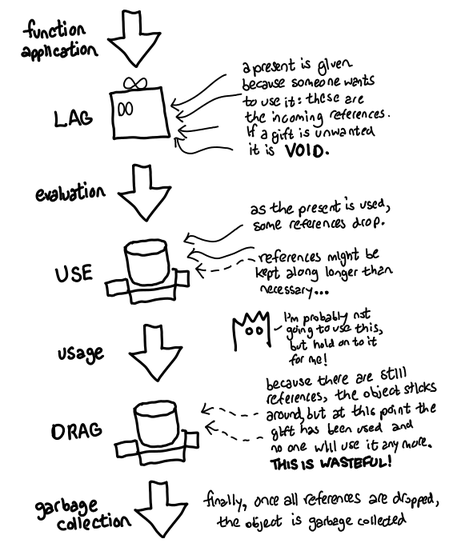
\includegraphics[width=5cm]{img/2023-05-24_16-21-37_screenshot.png}
\caption{\label{fig:orgd5445da}A general overview of the steps of garbage collection \autocite{yangHowGrinchStole}}
\end{figure}

\paragraph*{Newly generated data}
\label{sec:org732cdca}

When new data are generated, they are stored in the \emph{nursery}, a 512kb memory space \autocite{haskellwikiHaskellHaskellWiki2023}. In every iteration of the garbage collector, each value in Gen 0 that is still used is promoted in Gen 1\footnote{The transition to Gen 1 actually involves two steps: Data that are not to be deallocated remain in Gen 0 during the ``aging'' phase, before being promoted to Gen 1.}.

\begin{figure}[htbp]
\centering
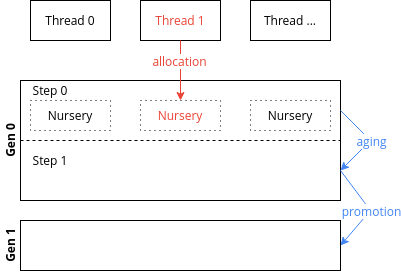
\includegraphics[width=8cm]{img/2023-05-24_15-45-31_screenshot.png}
\caption{\label{fig:orgedd7dd8}Two-generation GC of \texttt{ghc} \autocite{channableLessonsManagingHaskell}}
\end{figure}

\paragraph*{Collecting the garbage}
\label{sec:org16d89de}

The garbage collector initiates a search, starting from the so-called \emph{roots}, meaning the data in the stack and possible global variables. It then moves towards any data that roots point to. These pieces of data are stored in the heap.

\paragraph*{Copying}
\label{sec:org1e6f64c}

The visited pieces of data are then copied in parallel to a newly allocated heap \autocite{marlowParallelGenerationalcopyingGarbage2008} (figure \ref{fig:org8e10e07}). This process is called ``evacuation'' \autocite{yangHowGrinchStole}.

\begin{figure}[htbp]
\centering
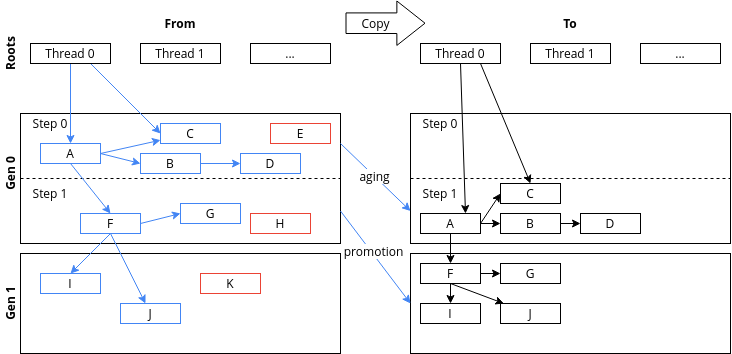
\includegraphics[width=8cm]{img/2023-05-24_16-16-17_screenshot.png}
\caption{\label{fig:org8e10e07}The copy mechanism of the \texttt{ghc} GC \autocite{channableLessonsManagingHaskell}}
\end{figure}

``Parallel'' means that as the GC searches for the data that the roots are pointing to, the roots are ``migrated'' in the new heap at the same time. The process of finding the data pointed by the roots is called ``scavenging'' \autocite{yangHowGrinchStole}.

Also, if a piece of data is evaluated and its value is used, it is then considered garbage and collected by the GC \autocite{yangHowGrinchStole}.

The downsides of this copying property of the GC is that the memory needed is double the one of the initial heap. That is, the old heap can't be freed before all of its live data are copied in the new heap.

This problem is solved by the use of a mark-compact algorithm, that reduces memory needs by rearranging the live data in the same heap \autocite{channableLessonsManagingHaskell}. It is used when there are a lot of live data in the old heap.

\paragraph*{Compact regions}
\label{sec:org62cd003}

Another problem of the garbage collection in Haskell is that it is performed successively with the main thread and not in parallel. That means that the process of garbage collection halts the running program and therefore time complexity is afflicted\footnote{From version 8.10 of \texttt{ghc} there exists an alternative GC strategy that allows concurrency \autocite{gamari972ConcurrentGarbage2019}.} \autocite{channableLessonsManagingHaskell}.

The solution to the previous problem is found in \emph{compact regions} \autocite{yangEfficientCommunicationCollection2015}, which were introduced in version 8.2.1 of \texttt{ghc}. They constitute a section of memory that is treated as a separate heap and handled separately. If, while searching, GC encounters data that lives in a compact region, then it stops searching for dead data pointed by it. This function is better illustrated in figure \ref{fig:org85fee36}. By using compact regions to store big amounts of live data, garbage collection time is greatly reduced. Compact regions are pinned in memory and the GC doesn't alter them in any way \autocite{channableLessonsManagingHaskell}.

\begin{figure}[htbp]
\centering
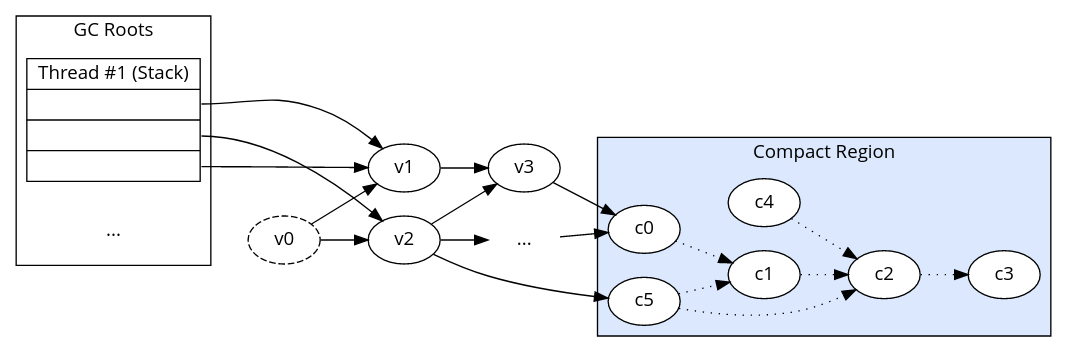
\includegraphics[width=8cm]{img/2023-05-24_16-44-12_screenshot.png}
\caption{\label{fig:org85fee36}Compact regions in GC \autocite{channableLessonsManagingHaskell}. When the GC reaches c0, it stops searching for dead data in anything that is pointed by it. As a result, data such as c4 is kept, even though nothing points to it.}
\end{figure}

\paragraph*{Mutability and garbage collection}
\label{sec:org5a1a4b7}

Mutability is one of the features of Haskell that negatively influences GC time. Mutability gives data the ability to point to ``future'' objects, meaning data that have not yet being created. This means that a live object in Gen 0 can depend in an object of Gen 1 \autocite{channableLessonsManagingHaskell}.

\subsection{Namespaces}
\label{sec:org8845d5c}

\subsubsection{Definition}
\label{sec:orgffdaff0}

A namespace is group of related elements that each one of them has a unique name so it can be easily identified\footnote{\url{https://techterms.com/definition/namespace}}.

\subsubsection{Namespaces in Haskell}
\label{sec:org74ffadd}

In Haskell there are 6 kinds of names that can be grouped in broader categories as follows: Firstly, Values. They consist of variables and constructors. Second, Entities related to file system. They consist of type variables, type constructors and type classes. Third and last, Modules. They consist of module names.

Haskell has just 2 naming constraints: First, names for variables and type variables are the only names that start with underscore or a lowercase letter. The names for the other categories are not allowed to start with these characters. Second, a class and a type constructor cannot use the same identifier as a name in the same scope \autocite{marlowHaskell2010Language2010}.

\subsection{Parallelism and Concurrency}
\label{sec:org0dcf542}

\textbf{Parallelism} and \textbf{Concurrency} are two different concepts in Haskell that enable the execution of tasks concurrently or in parallel, allowing for increased performance and more efficient utilization of hardware resources. Haskell provides exceptional support for both of them.

Parallelism indicates to the execution of computations simultaneously on multiple cores, while Concurrency refers to managing multiple tasks concurrently, without regard to the number of physical processors. Haskell's libraries like \texttt{Control.Parallel} and \texttt{Control.Concurrent} facilitate parallel and concurrent programming.

Haskell provides several mechanisms for parallel programming:

Annotations like \texttt{par} and \texttt{pseq} allow programmers to explicitly specify parallel or sequential execution. Using the par keyword the developer denotes that an expression can be evaluated in parallel, while \texttt{pseq} enforces sequential evaluation. The par annotation only acts as a guide to the runtime system, in order for it to evaluate expressions in parallel whenever possible.

\textbf{Strategies} are high-level abstractions for specifying parallelism. The \texttt{Eval} monad along with the \texttt{rpar} and \texttt{rseq} combinators provided by the \texttt{Control.Parallel.Strategies} module allow developers to express parallel computations more flexibly and easily. Strategies also enable you to specify granularity control, something truly important for load balancing and steering clear of excessive overhead.

Furthermore, there are parallel versions of common list functions, like \texttt{parMap} and \texttt{parList}, which automatically distribute the computation across processors. These functions make it convenient to parallelize operations on lists and apply a function to each one of the elements concurrently.

As it was already stated, Concurrency deals with managing multiple tasks, regardless of the underlying hardware capabilities. It mainly focuses on the organization and coordination of tasks to achieve efficient resource sharing and responsiveness. Haskell provides several powerful abstractions and features for managing concurrency in a safe and expressive manner.

The \texttt{IO} monad provides input/output operations, including concurrent I/O. It ensures that I/O actions are sequenced correctly and provides a safe and controlled scheme to perform concurrent operations.

Software Transactional Memory (STM) is a powerful mechanism for managing shared mutable states. It allows multiple threads to perform transactions, which are sequences of operations on shared memory. It ensures that transactions are atomic and isolated, preserving data integrity and simplifying concurrent programming. STM makes concurrent programming easier by automatically handling conflicts (race conditions - false sharing) and providing a consistent view of shared data.

Haskell enables developers to write concurrent programs that are concise, scalable, and robust.

\subsection{Metaprogramming}
\label{sec:orga39d03b}

\textbf{Metaprogramming} in Haskell refers to writing programs that manipulate other programs as data. It allows programmers to generate, transform, and analyze Haskell code.

Haskell provides various features for metaprogramming:

\textbf{Template Haskell} is a prominent metaprogramming extension built into \texttt{ghc}. It grants developers the capability to define and manipulate Haskell syntax at compile-time. With Template Haskell, dynamic code generation, code transformations and embed domain-specific languages (DSLs) are all possible within the language.

\textbf{Quasi-quotation} is another metaprogramming technique in Haskell. It allows code written in a different language or DSL to be directly embedded within Haskell source code. It provides a simplified way to generate or manipulate code in a non-Haskell language.

Haskell's strong type system enables type-level programming, writing code at the type level. It also allows for performing computations and expressing complex constraints at compile-time. Type families, type-level functions, and type-level literals are the tools that support type-level programming in Haskell.

Metaprogramming in Haskell serves various purposes, such as code generation to automate repetitive or boilerplate code, creating domain-specific languages for concise and expressive abstractions, transforming programs in order to be optimized and adaptive to specific requirements as well as enabling generic programming for code reuse across different data types. While metaprogramming can be a potent technique, it must be based upon a deep understanding of Haskell. Extreme care is needed, in order to maintain code clarity and readability when using metaprogramming approaches.

\subsection{Object-Oriented Properties of Haskell}
\label{sec:org1465a40}

Haskell is a functional language and as a result it does not provide object oriented functionalities by default. However, there are some tools given by the language that can be used to encode object oriented features in it \autocites{frankObjectorientationHaskellExploring2013}[][]{kiselyovHaskellOverlookedObject2005}. A sample representation of two fundamental entities of Object Oriented Programming follows: Classes and Objects.

\subsubsection{Classes}
\label{sec:orge035bcc}

A class can be mapped to an abstract Haskell type. A constructor can be defined as well, as it is supported by Haskell. Lastly, the user can define the needed functions that use that type \autocite{frankObjectorientationHaskellExploring2013}.

\begin{listing}[htbp]
\begin{minted}[]{csharp}
class C {
    C(int x) { ... };      /*Constructor*/
    static int s(int x);   /*Static method*/
    int m(bool b, int x);  /*Instance method*/
}
\end{minted}
\caption{\label{lst:org27c525e}A class definition in C\#}
\end{listing}

\begin{listing}[htbp]
\begin{minted}[]{haskell}
newtype C  -- An abstract type
newC :: Int -> IO C
s    :: Int -> IO Int
m    :: (Bool, Int) -> C -> IO Int
\end{minted}
\caption{The equivalent ``class'' in Haskell (listing \ref{lst:org27c525e})}
\end{listing}

\subsubsection{Objects}
\label{sec:org3a60507}

The objects of a class can be modeled as containers (data structures) that contain the data of the class. In Haskell the user has to define the data structure in two phases: data declaration and a class declaration for its methods \autocite{frankObjectorientationHaskellExploring2013}.

\subsubsection{Conclusion}
\label{sec:orgb74f977}

To conclude, Haskell does not provide native object-oriented functionalities, but most of them can be implemented in the language.

\subsection{Classes}
\label{sec:orgbe42ecb}

\begin{figure}[htbp]
\centering
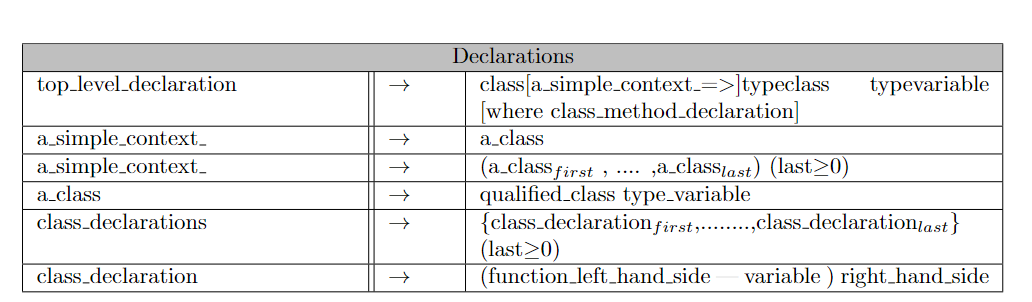
\includegraphics[width=.9\linewidth]{img/2023-05-25_13-28-35_screenshot.png}
\caption{\label{fig:orga5ad406}Classes in Haskell}
\end{figure}

In Haskell a new class can be defined alongside with its operations through the process of class declaration. The syntax \mintinline{haskell}{class cx=> MyClass tv where dec} is a way to declare a class. \texttt{MyClass} is the name of the new class, and \texttt{tv} is a type variable that is used only within the class definition. Also The \texttt{cx} part of the declaration specifies any superclasses of \texttt{MyClass}. Finally, the \texttt{dec} part of the declaration specifies the methods and properties that belong to the class \autocite[chapter 4.3]{marlowHaskell2010Language2010}.

Specifically from the class declarations we have the following: A class declaration results in the creation of class methods, represented b variables\textsubscript{i}. The class methods defined within the class declaration are not limited to the class declaration itself, but can be accessed and used outside of it. Every class method will have this kind of type, \mintinline{haskell}{method :: context => type}.

In Haskell, it is known that types like variables, functions, data types etc. have the same namespace. This basically means that two different top-level names can't have the same name because of the conflicts that may occur.

The same rule also applies for classes and their bindings. A compilation error will happen when there are two or more names with the same identifier in the same namespace. So the following is the signature form of a top level class method: \texttt{fn ::} \(\forall x, y. (Cx, cyz) \rightarrow r\).

Type classes provide a way to abstract over container types, allowing class methods to have polymorphic type signatures that can involve additional type variables and constraints beyond the primary type parameter of the class (listing \ref{lst:org0d6e103}).

\begin{listing}[htbp]
\begin{minted}[]{haskell}
class Container c where insert :: a -> ca -> c a
remove :: a -> ca -> c a
size :: c a -> Int
\end{minted}
\caption{\label{lst:org0d6e103}Polymorphic type signatures}
\end{listing}

Also, fixity declarations are used to specify the precedence and associativity of operators \autocite{marlowHaskell2010Language2010}. It is possible that the \texttt{dec} declaration from above has fixity declarations for class methods, allowing to specify the precedence and associativity of those methods.

Finally, in Haskell a default class method is a method that provides a default implementation. It is offered for a class method in case it is not defined explicitly in an instance declaration. In Haskell, a class declaration can have a \texttt{where} keyword, which contains the method signatures for the class methods. A class declaration may also not have this \texttt{where} keyword. The second case is used in order to merge many classes to one bigger class that inherits the methods of the smaller ones (listing \ref{lst:orgbafa18b}).

\begin{listing}[htbp]
\begin{minted}[]{haskell}
class (Ord a, Num a) => OrderedNum a where
absSquared :: a -> a
\end{minted}
\caption[Class inheritance]{\label{lst:orgbafa18b}Class inheritance. In this example, the \texttt{OrderedNum} class combines the \texttt{Ord} and \texttt{Num} classes and defines a new method \texttt{absSquared} that is specific to \texttt{OrderedNum} instances.}
\end{listing}

Becoming an instance of a subclass is not guaranteed. Mainly if a type is an instance of the superclasses. To make a type an instance of such a subclass, then an explicit instance definition without a \texttt{where} must be given \autocite{marlowHaskell2010Language2010}.

\subsubsection{Instance Declaration}
\label{sec:orgde9d300}

\begin{figure}[htbp]
\centering
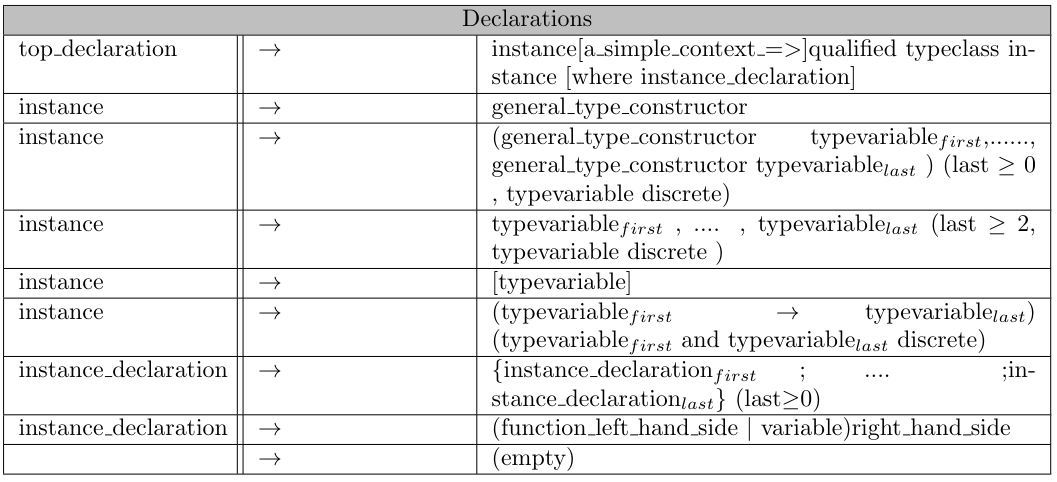
\includegraphics[width=.9\linewidth]{img/2023-05-25_18-46-02_screenshot.png}
\caption{Instance declarations}
\end{figure}

An instance declaration, on the other hand, defines an implementation of a class for a specific type.

\begin{minted}[]{haskell}
class (constraint) => Aclass parameter where cbody
\end{minted}

The following instance declarations cannot be used.

\begin{minted}[]{haskell}
instance Aclass (typ,typ) where ...
instance Aclass (Int,typ) where ...
instance Aclass [[typ]] where ...
\end{minted}

From the above examples tuple types which their elements have the same types are not allowed to be used by an instance declaration. Also it is not allowed to have the first element as a specific type and the second element as a type variable. Finally an instance cannot use a list of lists of type variables.

A class declaration provides type signatures and fixity declarations so they are not allowed in an instance declaration. The method declarations within the instance must be in some kind of forms. These forms must be in the form of a variable or function definition.

When a class method is not explicitly bound in an instance declaration, Haskell looks for a default
class method. If a default is found, it is used in place of the missing binding \texttt{else}, Haskell assigns the
value to \texttt{undefined}, which will not trigger a compile-time error \autocite{marlowHaskell2010Language2010}.

In order to declare an A-B instance that A is an instance of the class B then a number of constraints must be satisfied:

\begin{enumerate}
\item In Haskell, you cannot define a type as an instance of a given class many times in a program.

\item Kind inference can be used in order to make the class and type have identical kind. Those two must have the same type.

\item Hypothetically there’s an instance context \texttt{con 0}, which restrictions are satisfied by the \(b_{}k\) of the instance type \(A(b_1, \dots, b_{}k)\). Then the following rules must be satisfied as well:

\begin{itemize}
\item The restrictions provided by the superclass context \texttt{con0} of a class declaration should not be violated.

\item In order to get the class method declarations presented the correct way, then the restrictions on the type variables must not be violated as well.
\end{itemize}
\end{enumerate}

\begin{minted}[]{haskell}
class Animal b => Mammal b where ...
instance (Eq b, Show b) => Animal [b] where ...
instance Num b => Mammal [b] where ...
\end{minted}

In the above example the \texttt{Mammal} is a subclass of \texttt{Animal} so the second declaration is acceptable if \texttt{[b]} is an instance of \texttt{Animal}. \texttt{Eq} and \texttt{S} are superclasses of \texttt{Num} so the \texttt{[b]} is an instance of \texttt{Animal} from the first declaration.

On the other hand, if there are two instance declarations

\begin{minted}[]{haskell}
instance Num b => Mammal [b] where ...
instance (Eq b, Show b) => Animal [b] where ...
\end{minted}

The program wouldn't be acceptable. In order to be acceptable then for the second instance it is required that the \texttt{[b]} has to be instance of \texttt{Mammal}, including the fact that this should happen including \texttt{Eq b} and \texttt{Show b}. However in this case it is not true.

\subsubsection{Derived Instance}
\label{sec:orgf3eaa0b}

A deriving keyword can be included when defining a data type or a new type. This keyword makes the following difference: basically this move gives permission for a automatic creation of instance declarations for this type. This happens in specific classes. It must be noted that the generated instances have identical limitations as other instances (user-defined). The derivation of a class can happen when instances for the class’s superclass are present, and they actually do exist. It can happen through the definition of a distinct instance declaration or by adding the superclass in the clause that the derivation happens.

There are many benefits that come from a derived instance. One of them is a simple approach to defining operations that are used all the time (referring to custom data types). Instead of defining these operations from scratch, the derived instances for datatypes in the class \texttt{Eq} define them for the programmer. This can save time and effort and can help ensure consistency in the implementation of these operations.

Only for a specific set of classes can derived instances be permitted (\texttt{Eq}, \texttt{Ord}, \texttt{Enum}, \texttt{Bounded} etc.). The standard libraries’ defined classes can be eligible for derivation as well.

If a class name is included in a deriving form and the generation of an instance declaration cannot happen, then there’s an error \autocite{marlowHaskell2010Language2010}. Additionally, if a class is both explicitly declared and derived, this will also result in an error.

\subsubsection{Defaults, ambiguous types}
\label{sec:org141e7d9}

top level declaration \(\rightarrow \text{default} (\text{just}\_\text{a}\_\text{type}_{\text{first}}, \dots, \text{just}\_\text{a}\_\text{type}_{\text{last}})\).

In Haskell, ambiguous types can be the result of an overloading implementation. Supposing there’s a
typeclass named \texttt{MyClass} with a single function \texttt{Func} (like in the following listing).

\begin{minted}[]{haskell}
class MyClass a where
Func :: a -> Int
\end{minted}

Also there are definitions of two instances of \texttt{MyClass} for \texttt{Typea} and \texttt{Typeb}:

\begin{minted}[]{haskell}
instance MyClass Typea where
Func x = 1

instance MyClass Typeb where
Func x = 2  
\end{minted}

The use of \texttt{Func} with an ambiguous type like this here: \mintinline{haskell}{let x = Func undefined in ...} will have as a result a type error, because Haskell doesn't know what instance to use, \texttt{Typea} or \texttt{Typeb} for Func based on the type of undefined.

We have an ambiguous type when a type of an expression contains a type variable that appears in the
context but it isn't in the result type. For example, suppose we have a function \texttt{Func} with the following type signature:

\begin{minted}[]{haskell}
Func :: Num a => a -> a -> a
\end{minted}

Also there’s this use:

\begin{minted}[]{haskell}
let x = Func 5 6 in show x
\end{minted}

Here, the type of \texttt{x} could be any type that is an instance of \texttt{Num}, which includes \texttt{Int}, \texttt{Double}, \texttt{Float}, and others. Since \texttt{show} can work with any type that is an instance of \texttt{Show}, the type of the expression \texttt{show x} is ambiguous, because it could be any of the possible types that \texttt{x} could have.

In order to resolve such a problem we use an expression type like this:

\begin{minted}[]{haskell}
let x = Func 5 6 in show (x :: Int)
\end{minted}

the type of \texttt{show} is unambiguous here.

In order to ensure that an ambiguous expression has identical type with a variable, the use of the
function \texttt{asTypeOf} can be helpful.

To address the most frequent ambiguities arising from the \texttt{Num} class in Haskell, the language gives an alternative method known as \emph{default declaration}. The form of it is \(\text{type}_{\text{first}}, \dots, \text{type}_{\text{last}} \text{last} \geq 0\). An ambiguous type is \emph{defaultable} if the following are valid (supposing there’s an ambiguous type variable \texttt{x}):

\begin{enumerate}
\item Supposing we have the form \texttt{Class x} where \texttt{Class} is a class. If \texttt{x} occurs only in those kind of type constraints then it is defaultable.
\item If there is one class among the constraints that is a subclass of or equivalent to the \texttt{Num} class, then it is considered as a ``numeric class'' (the \texttt{Num} class is the most common numeric class in Haskell, and it defines basic numeric operations such as addition, subtraction, multiplication, and negation).
\item The classes in which the type variable \texttt{x} appears should be either in the Prelude or in a standard library.
\end{enumerate}

A defaultable variable can be substituted by the type that is mentioned as first (noting that it is in the default list) that satisfies all of its classes.

It is also worth noting that each module can have a single default declaration. Also its scope is bounded to that module. The cases that default types are assumed (specifically \texttt{Integer}, \texttt{Double}) are the cases where a default declaration is not explicitly provided.

\subsection{(Trans)portability}
\label{sec:org7b9e4ba}

The implementation of Haskell, also known as \texttt{ghc}, is supported by a variety of platforms. These platforms are divided into three tiers, as indicated by the \texttt{ghc} GitLab repository's wiki \autocite{gamariPlatformsGlasgowHaskell2023}.

\begin{itemize}
\item Tier 1

Tier 1 comprises major computing platforms, such as Windows (MinGW), MacOS X, and Linux, supporting x86/64, x86, and AArch64 architectures. The \texttt{GHCi} interpreter, \texttt{NGC} native code generator, and dynamic libraries are all supported in these platforms. To be included in tier 1, a platform must satisfy certain requirements, including the availability of a GitLab CI runner and a dedicated sponsor to provide support for new releases \autocite{gamariPlatformsGlasgowHaskell2023}.

These platforms constitute the main targets for \texttt{ghc} developers. All platforms in tier 1 must be supported to release a new version of \texttt{ghc}.

\item Tier 2

Platforms on tier 2 consist largely of various BSD distributions such as FreeBSD and OpenBSD, Solaris, and some less typical architectures of Linux. There is varying support for the \texttt{GHCi} interpreter, \texttt{NCG}, and dynamic libraries for these platforms. Support for these platforms depends heavily on community support, since \texttt{ghc} is open-source software. Therefore, not all platforms in tier 2 may necessarily be supported by new releases of \texttt{ghc}.

\item Tier 3

Finally, tier 3 includes platforms such as iOS, AIX, and the RISC-V architecture version of Linux. These platforms are less reliable, with some versions of \texttt{ghc} possibly available but generally unsupported.
\end{itemize}

\section{Examples and code}
\label{sec:orgd9d4a02}

\subsection{The ``Hello, World!'' program in Haskell:}
\label{sec:orgce97a4a}

\begin{listing}[htbp]
\begin{minted}[]{haskell}
main = putStrLn "Hello, World!"
\end{minted}
\caption{\label{lst:org2999a99}``Hello, World!'' program}
\end{listing}

The program in listing \ref{lst:org2999a99} defines a main function that uses the \texttt{putStrLn} function to print the string \texttt{Hello, World!} to the console.

To run this program, you can save it in a file with a \texttt{.hs} extension. Then compile and execute it from the command line using the commands shown in listing \ref{lst:orgf695027}.

\begin{listing}[htbp]
\begin{minted}[]{shell}
$ ghc hello.hs
$ ./hello
Hello, World!
$
\end{minted}
\caption{\label{lst:orgf695027}How to compile and run a program with the \texttt{ghc} compiler}
\end{listing}

The \emph{Hello World} program is traditionally the first program we write when learning a new programming language. In the world of functional programming we need something different to showcase the power of Haskell.

\subsubsection{Compilation process of the \texttt{ghc} compiler}
\label{sec:org2932fa5}

After you compile a Haskell program there will be 3 new files (listing \ref{lst:org9616e42}).

\begin{listing}[htbp]
\begin{minted}[]{shell}
$ ghc HelloWorld.hs
[1 of 1] Compiling Main ( HelloWorld.hs, HelloWorld.o )
Linking HelloWorld ...
$ ls
HelloWorld HelloWorld.hi HelloWorld.hs HelloWorld.o
\end{minted}
\caption{\label{lst:org9616e42}Files generated by \texttt{ghc}}
\end{listing}

The \texttt{HelloWorld} file is the executable and the \texttt{HelloWorld.o} is the object file. The \texttt{HelloWorld.hi} file is an \emph{interface file}. It contains information about the object file that \texttt{ghc} would need if you were to compile other modules, so that it would be able to link against that object file (said information cannot be stored in a standard object file).

You could say that the interface file is the equivalent of C's header files, only these are generated by \texttt{ghc} from the original Haskell source. Thus, the interface file is used when \texttt{ghc} compiles other modules, and the object file is used when linking all modules together to produce the executable. It is safe to delete the \texttt{.hi} and \texttt{.o} files once the executable is successfully generated, but keeping them helps in rebuilding and recompilation times after small changes.

\subsection{Factorials implementation in Haskell}
\label{sec:org5693ad8}

\begin{listing}[htbp]
\begin{minted}[]{haskell}
factorial :: Integer -> Integer
factorial 0 = 1
factorial 1 = 1
factorial n = n * factorial (n - 1)

main :: IO ()
main = do
    putStrLn "Enter a number:"
    n <- readLn
    putStrLn ("The factorial of " ++ show n ++
               " is " ++ show (factorial n))
\end{minted}
\caption{\label{lst:org3cc67c4}The program takes the number \texttt{n} as input, calculates and prints \texttt{n}!}
\end{listing}

The program in the listing \ref{lst:org3cc67c4} defines a main function that prompts the user to enter a number, reads the number from the console using the \texttt{readLn} function, computes its factorial using the \texttt{factorial} function, and prints the result to the console using the \texttt{putStrLn} function.

\begin{listing}[htbp]
\begin{minted}[]{shell}
$ ghc factorial.hs
[1 of 1] Compiling Main ( factorial.hs, factorial.o )
Linking factorial ...
$ ./factorial
Enter a number:
5
The factorial of 5 is 120
\end{minted}
\caption{Executing listing \ref{lst:org3cc67c4}}
\end{listing}

\subsection{Lambda functions}
\label{sec:org94154ae}

Real use of lambda functions, acting on lists.

\begin{listing}[htbp]
\begin{minted}[]{haskell}
-- Calculate the sum of a list of integers
sumList :: [Int] -> Int
sumList = foldr (+) 0
-- sumList = sum
  
-- Calculate the product of a list of integers
productList :: [Int] -> Int
productList = foldr (*) 1
-- productList = product

main :: IO ()
main = do
    -- Create an array of integers ranging from a to b (b included)
    -- let list = [a ..b]

    let list_a = [1.. 5]
    print list_a

    let list_b = [-4 .. 33]
    print list_b

    let myList = [1..10]
    putStrLn $ "list = " ++ show myList
    putStrLn $ "The sum of list is " ++ show (sumList myList)
    putStrLn $ "The product of list is " ++ show (productList myList)
    putStrLn $ "Max element of list is " ++ show (maximum myList)
    putStrLn $ "Min element of list is " ++ show (minimum myList)
\end{minted}
\caption{\label{lst:org7d8a9d4}Sum and product of an integer list}
\end{listing}

\begin{listing}[htbp]
\begin{minted}[]{shell}
[1,2,3,4,5]
[-4,-3,-2,-1,0,1,2,3,4,5,6,7,8,9,10,11,12,
 13,14,15,16,17,18,19,20,21,22,23,24,25,26,27,28,29,30,31,32,33]
list = [1,2,3,4,5,6,7,8,9,10]
The sum of list is 55
The product of list is 3628800
Max element of list is 10
Min element of list is 1
\end{minted}
\caption{Result of listing \ref{lst:org7d8a9d4}}
\end{listing}

As you can see in listing \ref{lst:org7d8a9d4}, Haskell provides a really easy way to create an new array with integers ranging from \texttt{a} to \texttt{b} (\texttt{b} included). Even high level languages like Python do not provide a similar feature. You can exclude \texttt{b} using the \texttt{..:} operator. These lambdas were implemented for demonstration purposes, Haskell already provides lambdas like \texttt{sum}, \texttt{product}, \texttt{maximum} and \texttt{minimum}.

The main function then creates a list called \texttt{myList}, calls the \texttt{sumList} function to calculate its sum using \texttt{foldr} and then prints out the result using the \texttt{putStrLn} function. The same thing happens for the \texttt{productList} function.

Note that we use the \texttt{show} function to convert the input list and the resulting sum to strings so that we can print them out using \texttt{putStrLn}.

\subsubsection{The \texttt{foldr} function}
\label{sec:org6ddc447}

In Haskell, \texttt{foldr} is a higher-order function that takes a binary function and an initial accumulator value and applies the binary function repeatedly to the elements of a list, starting from the rightmost element, and accumulating the result in the accumulator value. The type signature of \texttt{foldr} is shown in listing \ref{lst:orge6caa7d}.

\begin{listing}[htbp]
\begin{minted}[]{haskell}
foldr :: (a -> b -> b) -> b -> [a] -> b
\end{minted}
\caption{\label{lst:orge6caa7d}The \texttt{foldr} type signature}
\end{listing}

\begin{itemize}
\item The first argument is the binary function that takes an element of type \texttt{a} and an accumulator value of type \texttt{b}, and returns a new accumulator value of type \texttt{b}. The second argument is the initial accumulator value of type \texttt{b}. The third argument is the list of elements of type \texttt{a}.

\item \texttt{foldr} works by applying the binary function to the last element of the list and the initial accumulator value, producing a new accumulator value. It then applies the binary function to the second-to-last element of the list and the new accumulator value, producing another new accumulator value. It continues this process until it reaches the first element of the list, at which point it returns the final accumulator value.
\end{itemize}

\subsection{The \texttt{GHCi} Interpreter}
\label{sec:org05d9f61}

To start a \texttt{GHCi} session use the command \texttt{ghci} (listing \ref{lst:org726f80f}).

\begin{listing}[H]
\begin{minted}[]{haskell}
$ ghci
GHCi, version 9.2.7: https://www.haskell.org/ghc/  :? for help
ghci>
\end{minted}
\caption{\label{lst:org726f80f}Using the \texttt{ghci} interpreter.}
\end{listing}

Any \textbf{Haskell expression} can be typed at the prompt. The \texttt{ghci} interpreter will output the result.

\begin{minted}[]{haskell}
ghci> 1+1
2
ghci> let x = 1 in x / 3
0.3333333333333333
ghci>
\end{minted}

You can also bind values (or expressions) and functions to names.

\begin{minted}[]{haskell}
ghci> x = 10
ghci> x
10
ghci> x = 3
ghci> x
3
ghci>
\end{minted}

This is only supported in newer versions, since \texttt{GHC} 8.0.1. In older versions you are obliged to use \texttt{let} statement. Take note of the ability to overwrite \texttt{x}'s value.

Of course, you can also define new lambdas. Here is an example:

\begin{minted}[]{haskell}
ghci> x = 10
ghci> addx y = y + x
ghci> addx 1
11
ghci> x= 11
ghci> addx 1
11
ghci> addx y = y + x
ghci> addx 1
12
ghci> 
\end{minted}

As you can see, even though we overwritten the value x, the \texttt{addx} lambda seems to hold the previous value of \texttt{x}. Even reassignments are a complex topic in Haskell.

Here is how someone would define the factorial function as a lambda using \texttt{ghci}:

\begin{minted}[]{haskell}
ghci> factorial n = product [1..n]
ghci> factorial 10
3628800
ghci>
\end{minted}

\section{Conclusion}
\label{sec:org92ae777}

Haskell is a computer programming language renowned for its functional paradigm, type system, and purity, which distinguishes it from other programming languages \autocite{marlowParallelConcurrentProgramming2013}. Haskell has a rich and storied history that reflects an ambition to create a smarter, more efficient, and easier-to-use functional programming language. It has lived up to this ambition, continuing to evolve and gain popularity in various industries, such as finance, web development, and academia, where its distinctive features are especially valued.

One of the essential and most notable Haskell features is its strict type system. This characteristic eliminates some of the most typical errors and catches them early in the development process, ultimately reducing the costs attributed to debugging and streamlining the software development cycle. Such advantage surpasses mere typing as the system allows for better documentation and significantly enhances the readability of your code. Moreover, Haskell's compiler can detect a wide range of errors that would otherwise be challenging to catch \autocite{huttonProgrammingHaskell2007}. Such characteristics make Haskell especially useful in the development of high-integrity systems where the cost of failure is high.

Another crucial aspect of Haskell is its non-strict evaluation, which makes it different from other programming languages. Non-strict evaluation allows the expressions to remain unevaluated until they are required. It promotes efficiency, reducing unnecessary computations.

One of the most significant advantages of Haskell is its purity, meaning that Haskell functions have no side effects. Such characteristics make code more predictable, easier to understand, and reduce the complexity of debugging and detecting errors commonly encountered in impure languages \autocite{huttonProgrammingHaskell2007}.

Haskell has a highly flexible control structure, which allows for the creation of smaller and more readable codebases. Haskell uses unique identifiers that require less explanation and come naturally to the understanding of developers.

Haskell has a wide variety of operators that provide a wealth of functionality in a natural and mathematical way, which makes them easier to remember and apply to problems \autocite{huttonProgrammingHaskell2007}. Operators can also be composed to form a single function, an ability that sets Haskell apart from other programming languages. This ability offers a high degree of concision and expressiveness that can aid in the development of intricate software systems.

Lambdas and Monads are two of the most valuable Haskell features. Lambdas are anonymous functions that are declared using a backslash, allowing for flexible, on-the-fly function creations. Monads are a unique Haskell abstraction that facilitates the organization and composition of code for solving complex problems \autocite{marlowParallelConcurrentProgramming2013}.

Finally, the Haskell memory management and runtime are optimized to provide superior performance levels. Haskell uses garbage collection, eliminating memory leaks and other errors typical of languages that do not have garbage collection. This results in improved performance and more reliable software programs.

\printbibliography
\end{document}